% This must be in the first 5 lines to tell arXiv to use pdfLaTeX, which is strongly recommended.
\pdfoutput=1
% In particular, the hyperref package requires pdfLaTeX in order to break URLs across lines.

\documentclass[11pt]{article}

% Change "review" to "final" to generate the final (sometimes called camera-ready) version.
% Change to "preprint" to generate a non-anonymous version with page numbers.
\usepackage[final]{acl}

% Standard package includes
\usepackage{times}
\usepackage{latexsym}
\usepackage{amsmath}
\usepackage{amssymb}
\usepackage{booktabs}
\usepackage{listings}
\usepackage{multirow}
\usepackage{paralist}
\usepackage{enumitem}
\usepackage{xcolor} 
\usepackage{caption} 
% for nicer tables (\toprule, \midrule, etc.)
\usepackage{xcolor}               % for the ↪ symbol colour
\lstdefinestyle{prompt}{
  basicstyle=\ttfamily\scriptsize, % small fixed-width font
  breaklines=true,                 % wrap long lines
  breakindent=0pt,                 % no hanging indent
  columns=fullflexible,            % don't force monospace width
  frame=single,
  framerule=0.4pt,
  framesep=3pt,
  xleftmargin=0pt, xrightmargin=0pt,
  postbreak=\mbox{\textcolor{gray}{$\hookrightarrow$}\space} % mark wrapped lines
}
% for the floating algorithm environment
\usepackage{algorithm}
\usepackage{algpseudocode}

\usepackage{framed}
\newenvironment{dblleftbar}{%
  \def\FrameCommand{\vrule width .8pt \hspace{.6pt}\vrule width .4pt \hspace{8pt}}% choose the values as you like
  \MakeFramed {\advance\hsize-\width \FrameRestore}}%
 {\endMakeFramed}
\newenvironment{quotationb}%
{\begin{dblleftbar}\begin{quotation}}%
{\end{quotation}\end{dblleftbar}}


% For proper rendering and hyphenation of words containing Latin characters (including in bib files)
\usepackage[T1]{fontenc}
% For Vietnamese characters
% \usepackage[T5]{fontenc}
% See https://www.latex-project.org/help/documentation/encguide.pdf for other character sets

% This assumes your files are encoded as UTF8
\usepackage[utf8]{inputenc}
\usepackage{textgreek}
\usepackage{url}
% This is not strictly necessary, and may be commented out,
% but it will improve the layout of the manuscript,
% and will typically save some space.
\usepackage{microtype}

% This is also not strictly necessary, and may be commented out.
% However, it will improve the aesthetics of text in
% the typewriter font.
\usepackage{inconsolata}
%\usepackage{parskip}

%Including images in your LaTeX document requires adding
%additional package(s)
\usepackage{graphicx}

% If the title and author information does not fit in the area allocated, uncomment the following
%
%\setlength\titlebox{<dim>}
%Structure-to-Text and Back: High-Fidelity Synthetic Data Generation for Knowledge Graphs
% and set <dim> to something 5cm or larger.


% \usepackage[draft, todonotes={textsize=tiny}]{changes}
\usepackage[final, todonotes={textsize=tiny}]{changes}
 \definechangesauthor[name=Kamyar, color=black]{K}
 \definechangesauthor[name=Silvia, color=orange]{S}
 \definechangesauthor[name=Alessia, color=blue]{A}

\usepackage[final]{changes}  % uncomment to remove comments
\title{From Graph to Text and Back: 
%Guaranteeing 
Semantic Fidelity in Automated Industrial Knowledge Graphs}

\author{Kamyar Zeinalipour \and Silvia Severini \and Alessia Borghini \and Sara Cardarelli \and Marco Maggini \and Marco Gori \\
  Department of Information Engineering and Mathematics (DIISM) \\
  University of Siena, Italy \\
  \texttt{kamyar.zeinalipour2@unisi.it}}




\begin{document}
\maketitle

\begin{abstract}
Knowledge Graphs (KGs) are the backbone of reliable industrial data strategies, yet verbalizing them with Large Language Models (LLMs) often leads to unacceptable risks for high-stakes applications, such as hallucinations or omitted relations. To enforce strict semantic fidelity in KG-to-text generation, we introduce a self-supervised \emph{round-trip} pipeline. The system verbalizes KG triples into text and immediately attempts to reconstruct the original graph from that text; only verbalizations that enable perfect graph recovery are retained. This creates a closed feedback loop that guarantees the generated text is semantically equivalent to the source data. Experiments confirm that our automated round-trip consistency score correlates strongly with expert judgment, effectively acting as a scalable proxy for human review. Furthermore, we show that standard LLMs can bootstrap their own KG-extraction and generation capabilities by fine-tuning on this trusted synthetic data. Our approach yields significant improvements in triple-extraction accuracy and verbalization faithfulness without relying on costly manual annotation or massive teacher models, offering a practical path to deploying trustworthy, KG-grounded AI systems.
\end{abstract}


%\begin{abstract}
%Generating accurate natural language from structured data remains a major challenge in natural language generation (NLG). High-quality synthetic text significantly enhances downstream tasks such as knowledge extraction, semantic understanding, and structured data creation.
%We propose a novel two-stage approach to generate \textit{High-Fidelity} synthetic text that faithfully preserves the original semantic meaning of structured inputs. First, a decoder model generates coherent, semantically accurate text from trusted structured inputs, like Knowledge Graph (KG) triples. Next, a complementary model reconstructs structured data from this synthetic text, ensuring semantic fidelity through precise text-to-structure mapping.
%We rigorously evaluate semantic fidelity by measuring the similarity between the original structured input and the reconstructed data derived from synthetic text. Employing semantic metrics 
%(i.e., \texttt{e5}) 
%and lexical similarity measures,
%(e.g., \texttt{ROUGE})
%our method dynamically selects optimal synthetic outputs via iterative similarity feedback. 
%Experiments on KG-to-text tasks confirm a robust alignment between computational metrics and human assessments, demonstrating reliability.
%Fine-tuning 
%on 
%different LLaMA models,
%\texttt{LLaMA3.1(1B)}, \texttt{LLaMA3.2(3B)}, and \texttt{LLaMA2(7B)} 
%with  our synthetic data notably enhances their KG generation performance compared to baselines and, unlike traditional methods that rely on larger-to-smaller model training, our approach uniquely demonstrates gains from models fine-tuned on their own generated data.
%Although our experiments focus on KG triples, the approach is task‑agnostic and in principle extends to a broad range of information‑preserving representations.
%, ranging from conventional structured sources such as tables, relational databases, and ontologies to text‑as‑structure scenarios (e.g., summary$\leftrightarrow$expansion or paraphrase cycles). A systematic empirical study of these additional domains is left to future work.
%Code and datasets are publicly available.\footnote{Link omitted to preserve blind review.}
%\end{abstract}


\section{Introduction}

In the enterprise landscape, Knowledge Graphs (KGs) serve as the backbone of reliable data strategies, providing a structured source of truth for downstream applications \citep{shao2022structured, jiang2023structgpt, osuji2024systematic}. However, bridging the gap between this rigid structured data and user-friendly natural language remains a critical bottleneck for industrial adoption \citep{li2022faithfulness}. While Large Language Models (LLMs) offer fluency, they introduce a ``black box'' risk: state-of-the-art models frequently hallucinate entities or omit relations, posing unacceptable liability risks in precision-critical domains such as healthcare and finance \citep{rebuffel2022controlling, ji2023survey}. For industry, the challenge is not merely generating text, but guaranteeing its \textbf{semantic fidelity} without incurring the prohibitive cost of manual verification.

\paragraph{Problem statement.}
To address this reliability gap, we formulate the following question:
\begin{figure}[t]
    \centering
    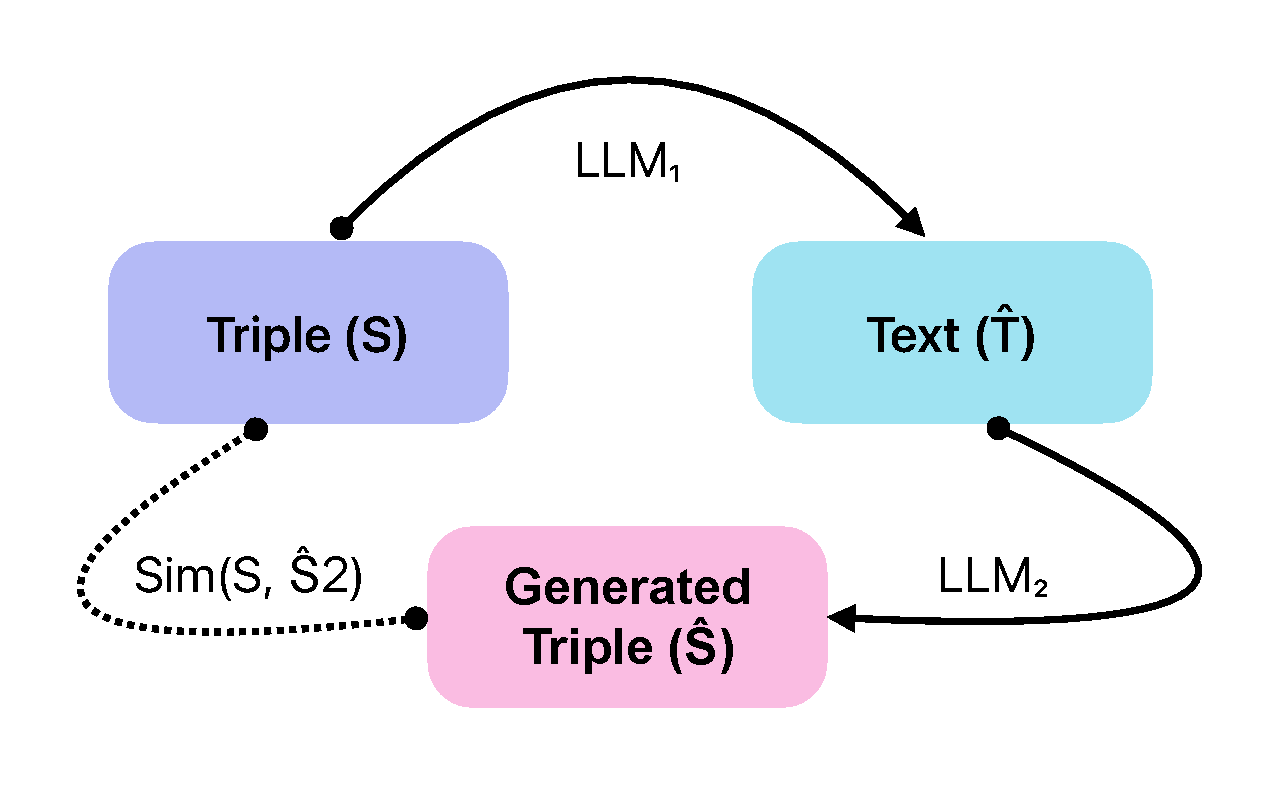
\includegraphics[width=0.9\columnwidth]{fig11.pdf}
    \caption{Overview of our proposed two-stage round-trip pipeline. Structured inputs ($S$) are verbalized into candidate texts ($\hat T$) (Stage~1), then reconverted to structured form ($\hat S$) (Stage~2). A similarity measure $\operatorname{sim}(S,\hat S, \alpha)$ evaluates the transformation quality.}
    \label{fig:approach-overview}
\end{figure}


\emph{How can we generate synthetic KG-to-text data that is guaranteed to be semantically equivalent to the source, enabling models to learn from their own output without human supervision?}

\noindent Solving this yields two distinct industrial advantages: (1) the creation of high-fidelity synthetic corpora without costly manual intervention, and (2) the establishment of a scalable, automated proxy for expensive Subject Matter Expert (SME) quality judgments.

\paragraph{Approach overview.}
We propose a two-stage round-trip pipeline (Figure~\ref{fig:approach-overview}). Stage~1 verbalizes a structured input $S$ into a candidate text $\hat T$; Stage~2 maps $\hat T$ back to a structured form $\hat S$. We compare the pair using a \emph{round-trip similarity} $\operatorname{sim}(S,\hat S, \alpha)$ combining embedding-based semantics and lexical overlap. A \textbf{dynamic-sampling controller} iteratively adjusts the decoding parameters to retain only candidates exceeding a target similarity. We illustrate this process in Figure \ref{fig:example} using a case study on the Komodo Dragon.
We investigate:
\begin{description}
\item[\textbf{RQ1}] Does $\operatorname{sim}(S,\hat S, \alpha)$ reliably track human ratings, serving as a scalable automated evaluator to replace manual review?
\item[\textbf{RQ2}] Can a model bootstrap its extraction accuracy by fine-tuning on its own high-fidelity synthetic text, thereby reducing the need for massive teacher models or labeled data?

\end{description}
\paragraph{Key findings.}
Across our 250-graph corpus, we find that:
(i)~the automatic score $\operatorname{sim}(S,\hat S, \alpha)$ aligns closely with human judgments, validating its use as a quality gate;
(ii)~self-training on this verified corpus boosts extraction quality on \emph{both} automatic metrics and blinded human studies, demonstrating a viable path for self-improving systems. 

\noindent \textbf{Contributions.} In summary, our contributions are:
(1)~an architecture-agnostic round-trip pipeline for producing \emph{high-fidelity} synthetic text from structured enterprise assets;
(2)~a similarity-driven dynamic-sampling mechanism that automatically calibrates decoding to ensure maximum semantic retention;
(3)~evidence that models can \emph{self-bootstrap} extraction performance via this pipeline, outperforming distillation baselines without manual labeling; and
(4)~the public release of code, checkpoints, and datasets.\footnote{Code and datasets available at \url{https://github.com/KamyarZeinalipour/round-trip-kg} under MIT license.}

\begin{figure}[t!]
\centering
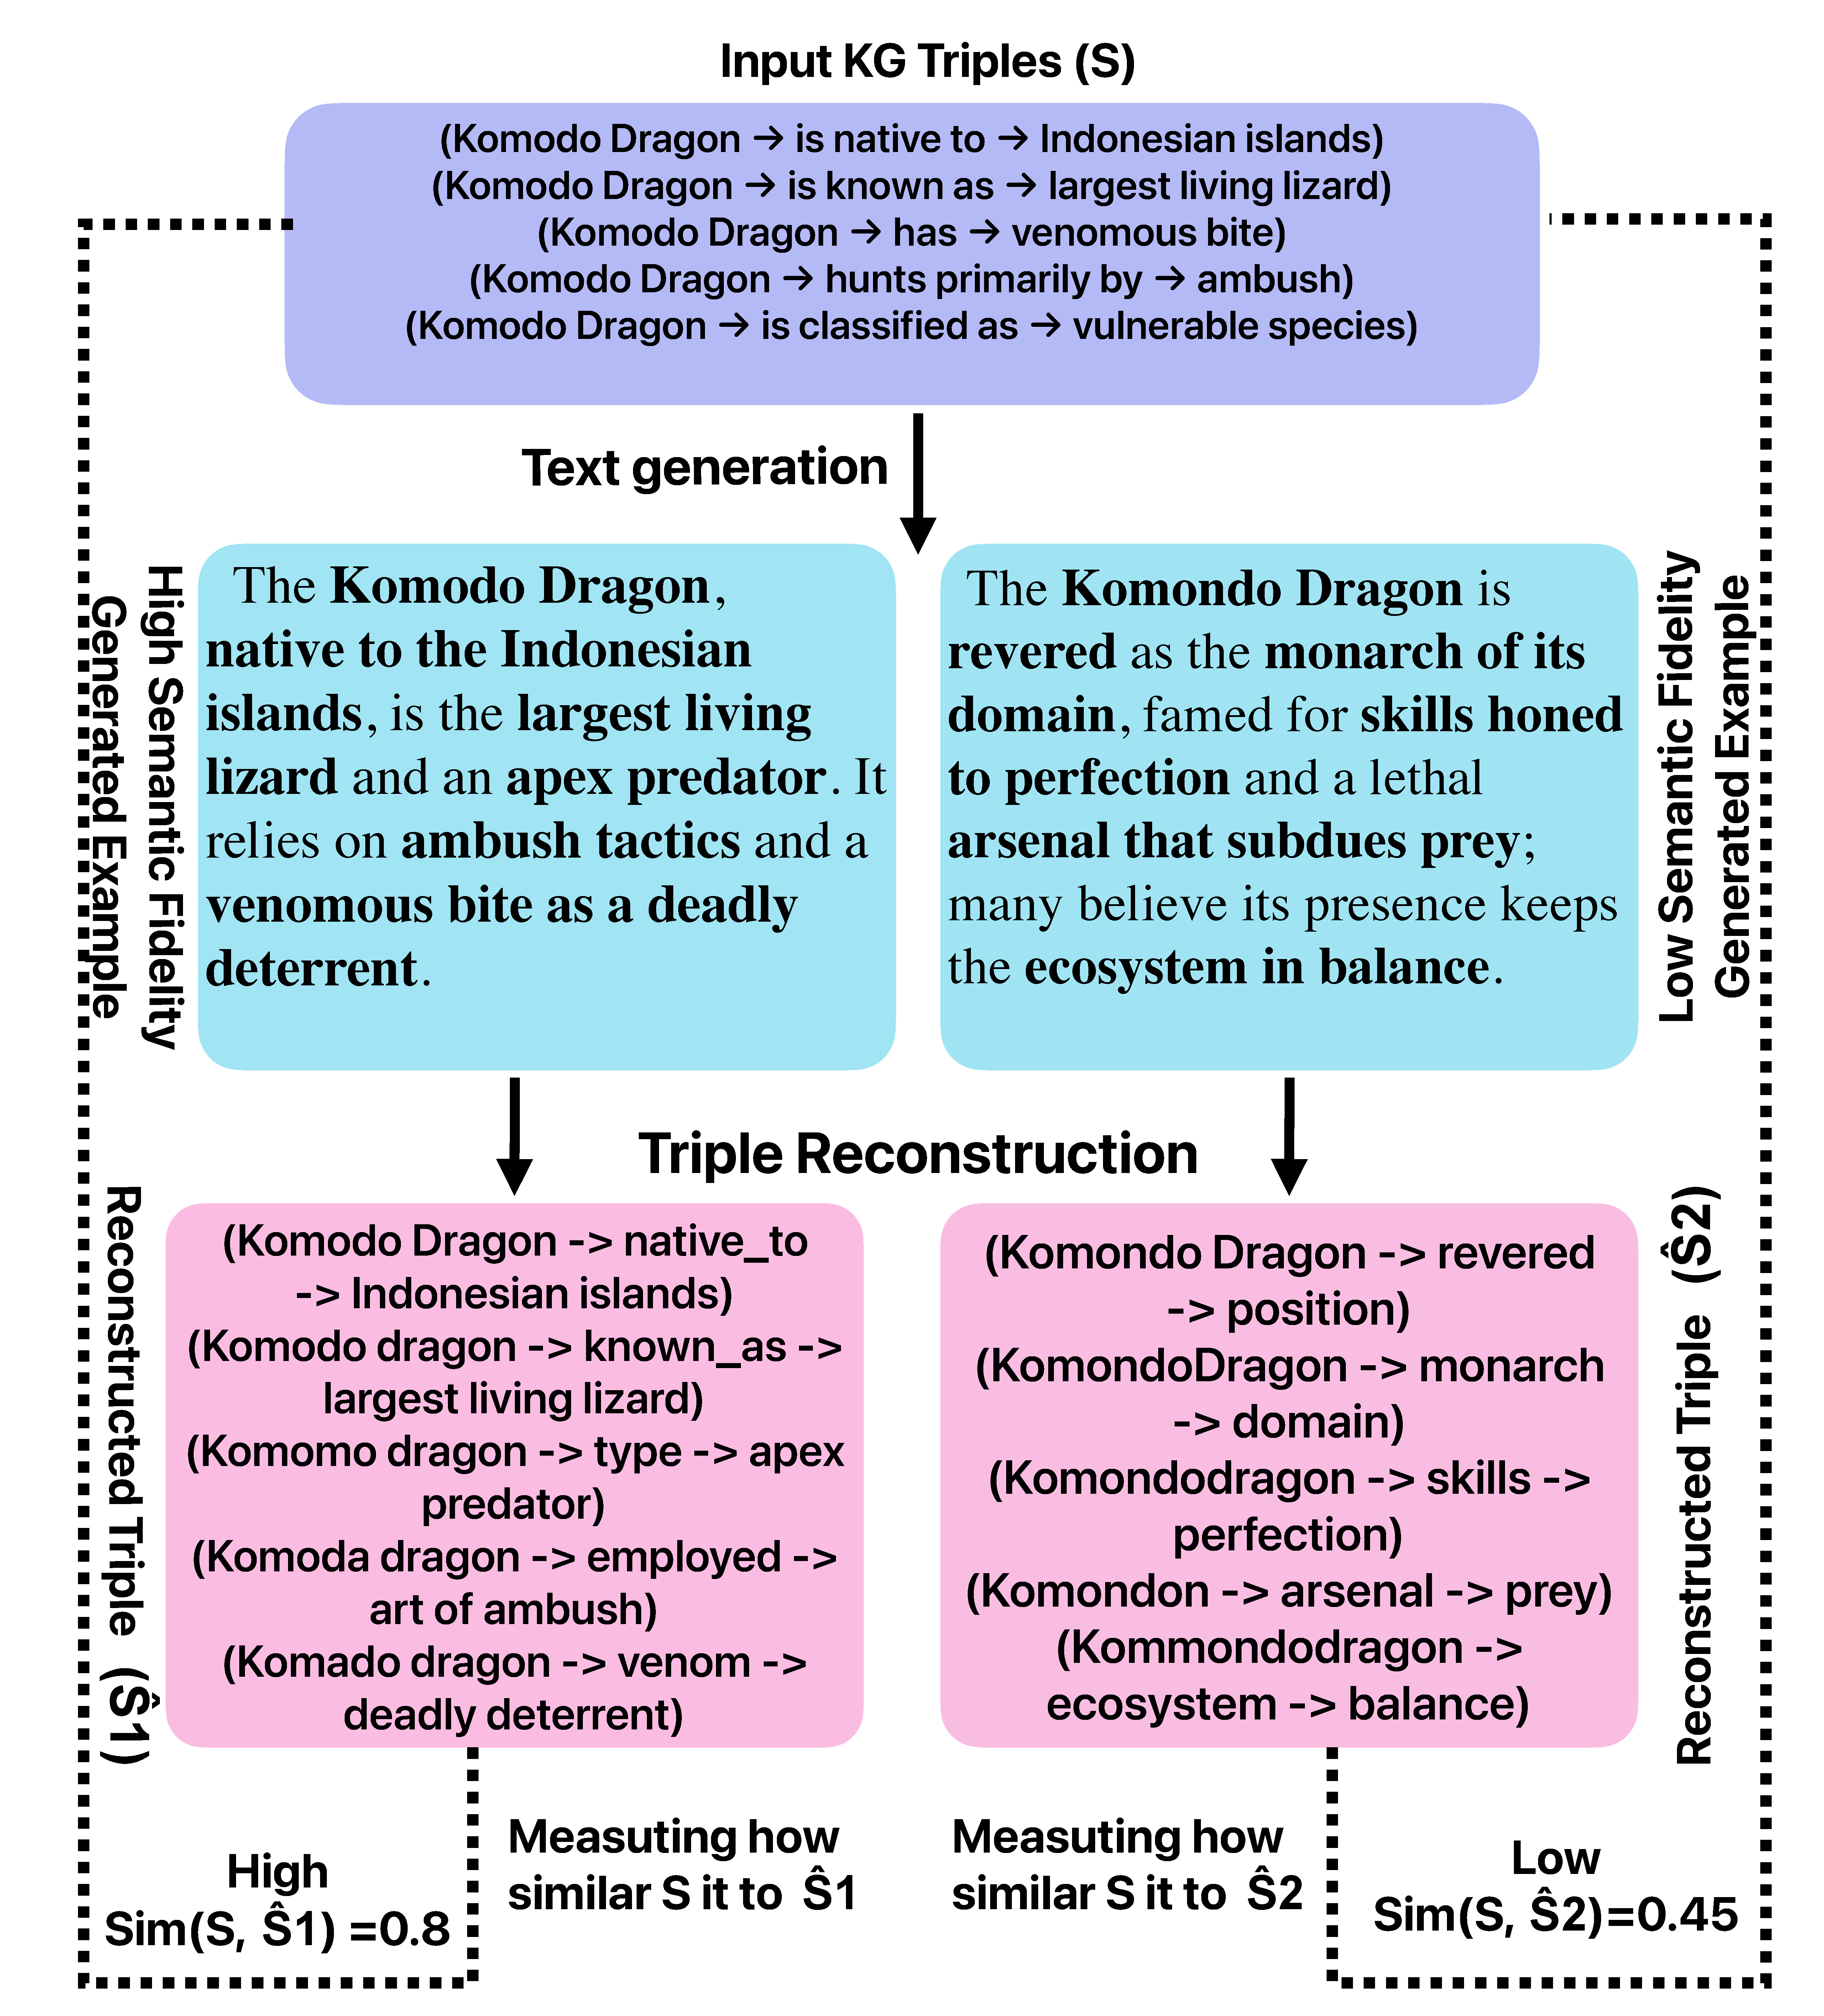
\includegraphics[width=\columnwidth]{example-dragon.pdf}
\caption{%
The input KG triples about the ``Komodo Dragon''  are first
           verbalized by the generator (Stage 1).
           The reconstructor then maps the text back to triples
           (Stage 2).  High-fidelity text (left) reproduces every fact,
           whereas a low-fidelity variant (right) introduces
           omissions and errors, leading to low round-trip similarity.\protect\footnotemark
           }
\label{fig:example}
\end{figure}
\footnotetext{We compressed the generated texts of Figure \ref{fig:example} to enhance visualization; the original text appears in the Appendix \ref{appendix:dragon_example}.}

\section{Related Work}

\paragraph{Risk Mitigation in Generative Systems}
Neural data-to-text systems frequently suffer from hallucinations and critical omissions \citep{Wiseman2017,Mei2016,Dusek2019,Thomson2020,Rebuffel2022}. Evaluation typically relies on n-gram overlaps \citep{Papineni2002,Banerjee2005,Lin2004} or coverage-aware metrics like \textsc{PARENT} \citep{Dhingra2019PARENT}. To ensure fidelity, prior work employs critic models \citep{Harkous2020,Lango2023Critic}, cycle-consistency losses \citep{Guo2020CycleGT,Gong2020TableGPT}, or specialized decoding strategies \citep{Holtzman2020Nucleus}. Our work operationalizes these insights via an automated back-parsing pipeline to guarantee high-fidelity outputs.

\paragraph{Scalable Data Synthesis \& Bootstrapping}
Synthetic data reduces annotation costs. To ensure high-quality data, round-trip methods have been used, such as back-translation \citep{Sennrich2016BT,He2016Dual} or unsupervised simplification \citep{Surya2019,Schumann2020}. In the LLM era, ``born-again'' networks and self-distillation \citep{Furlanello2018,Hinton2015} leverage self-instruction \citep{Wang2022SelfInstruct,Long2024Survey} and modern language capabilities \citep{radford2019language,liu2024best,long2024llms,bauer2024comprehensive} to bootstrap performance. Unlike teacher-dependent methods, we employ a self-contained loop filtering samples via embedding similarity \citep{Wang2023E5} to ensure semantic integrity.
\paragraph{Knowledge Graph-to-Text Systems}
KG-to-text has evolved from rule-based pipelines \citep{Reiter1997,Dale1998} to neural models, which often trade fidelity for fluency \citep{CastroFerreira2018,Mei2016,Wiseman2017}. Solutions range from specialized graph encoders \citep{Marcheggiani2018,KoncelKedziorski2019} and explicit planners \citep{Puduppully2019,Moryossef2019} to pre-trained integrations like JointGT \citep{Ke2021JointGT} and MGSA \citep{Wang2024MGSA}. Recent work emphasizes few-shot prompting \citep{Li2021FewShotKG,Zhang2024ChatGraph,Zhao2023KnowGPT} and large synthetic datasets \citep{kim2024ontology}. We complement these with a model-agnostic verification layer adaptable to standard LLMs.


\section{Methodology}
\label{sec:methodology}

We propose a domain-agnostic \textbf{structure-to-text-and-back loop} for generating synthetic text that faithfully retains input semantics. Demonstrated here with KG triples, the method generalizes to any structured representation as it relies on semantic consistency rather than task-specific constraints. The pipeline (Figure~\ref{fig:methodology}) comprises four steps: (1) Structure-to-Text Generation, (2) Text-to-Structure Reconstruction, (3) Iterative Refinement via Dynamic Sampling, and (4) Automated Selection. Algorithm~\ref{alg:loop} details this adaptive process.

\subsection{Workflow Overview}
\label{subsec:workflow}

\begin{figure*}[htbp]
    \centering
    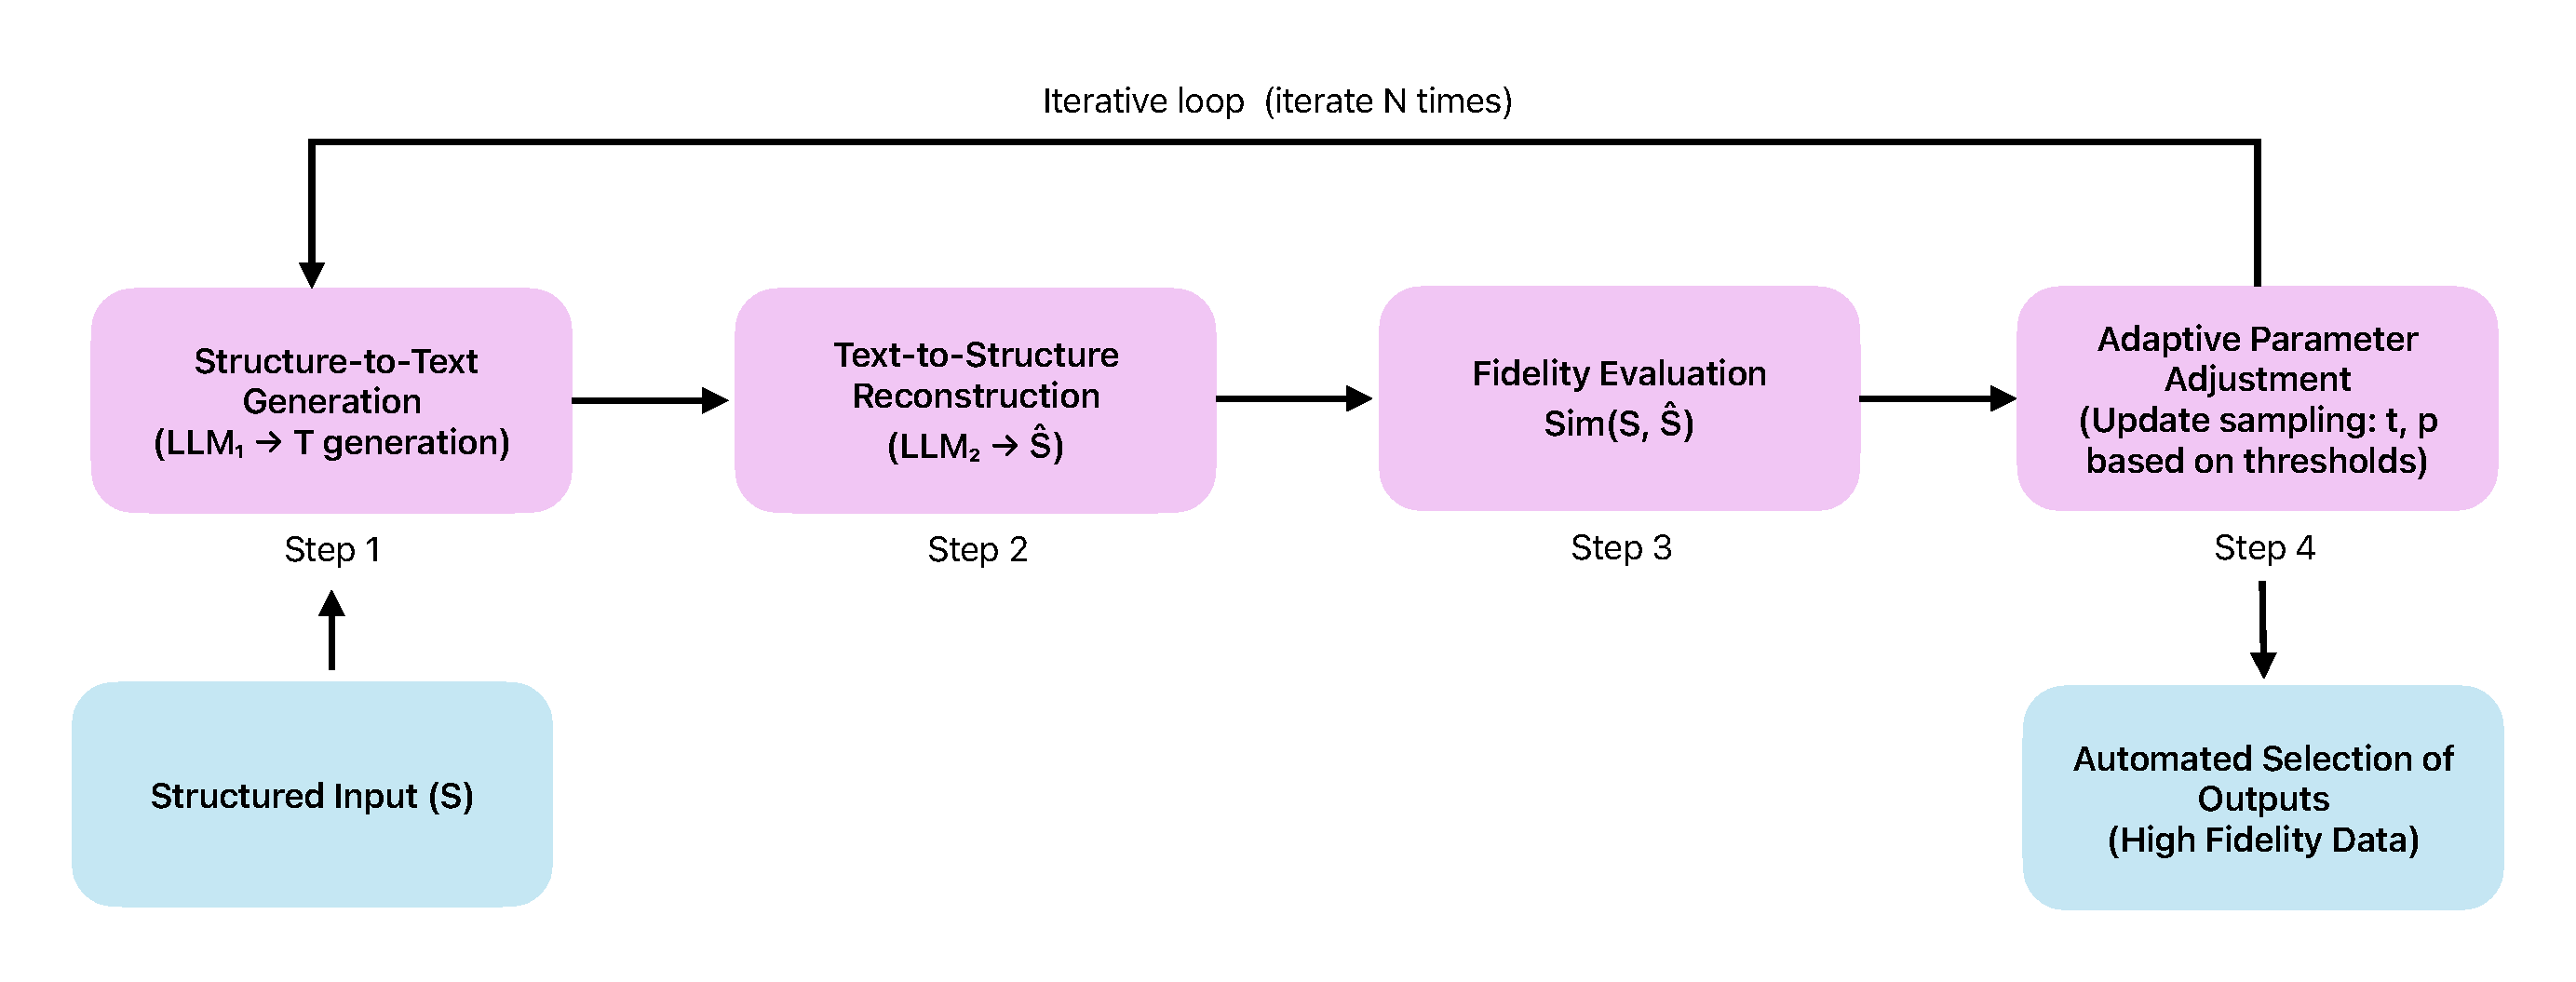
\includegraphics[width=0.95\textwidth]{method2_kg.pdf}
 \caption{Illustration of the iterative ``structure-to-text-and-back'' loop.
\textbf{Step 1 (Generation):} Structured inputs are converted into candidate texts by LLM$_1$.
\textbf{Step 2 (Reconstruction):} LLM$_2$ maps these texts back into structured form.
\textbf{Step 3 (Refinement):} Semantic and lexical similarity scores between the original and reconstructed data drive the adaptive adjustment of decoding parameters (temperature $t$, top-$p$).
\textbf{Step 4 (Selection):} Only outputs exceeding a high-fidelity threshold are retained.
The cycle repeats $N$ times to optimize synthetic quality.}
    \label{fig:methodology}
\end{figure*}


Given structured input $S$ (e.g., KG triples), the pipeline performs $N$ iterative cycles to generate text $\hat T$ and a structured reconstruction $\hat{S}$. Generation parameters are dynamically adjusted via the \textit{round-trip similarity}\footnote{Hyperparameters detailed in Appendix \ref{appendix:params_selection}.}.
The embedding function $\phi(\cdot)$ is implemented using \texttt{e5-mistral-large} \citep{Wang2023E5}, a state-of-the-art sentence encoder chosen for its ability to capture deep structural semantics regardless of surface phrasing---a critical requirement when comparing structured KG tuples against fluid natural language:
\[
\operatorname{sim}(S,\hat S, \alpha)=
\alpha \cdot \cos\bigl(\phi(S),\phi(\hat S)\bigr)
\;+
\]
\[
(1-\alpha)\cdot \mathrm{sim}_{\text{lex}}(S,\hat S)
\]
where $\phi(\cdot)$ represents embeddings, $\mathrm{sim}_{\text{lex}}$ is a lexical metric, and $\alpha \in [0,1]$ balances semantic and lexical alignment.\\

\noindent The workflow proceeds as follows:

\begin{enumerate}
    \item \textbf{Structure-to-Text Generation:} LLM$_1$ verbalizes structured data ($S$) into candidates ($\hat T$). To ensure diversity, subsequent iterations ($i \ge 3$) explicitly prompt the model to produce text distinct from previous versions, while the initial pass ($i=1$) generates directly. 

    \item \textbf{Text-to-Structure Reconstruction:} A complementary LLM$_2$ converts $\hat T$ back into structured format $\hat{S}$ to measure the semantic preservation of the transformation.

    \item \textbf{Iterative Refinement:} We evaluate fidelity via round-trip similarity and dynamically adjust decoding temperature ($t$) and top-p ($p$) to balance consistency and diversity:
 \[(t, p)\leftarrow(t,p)+
\]
\[
\begin{cases}
(-\Delta t,-\Delta p), & \operatorname{sim}(S,\hat{S}, \alpha)<\tau_{\text{low}};\\[2pt]
(0,0), & \tau_{\text{low}}\le \operatorname{sim}(S,\hat{S}, \alpha)<\tau_{\text{high}};\\[2pt]
(+\Delta t,+\Delta p), & \operatorname{sim}(S,\hat{S}, \alpha)\ge\tau_{\text{high}}.
\end{cases}
\]

    Thresholds and increments are tuned on the development set. This mechanism reduces randomness to recover fidelity when scores are low, and increases it to promote diversity when scores are high.

    \item \textbf{Automated Selection:} After $N$ cycles, outputs surpassing a strict threshold $\tau_{select}$\footnote{Determined via grid-search on the dev set.} are automatically retained, yielding a high-fidelity synthetic dataset without human intervention.
\end{enumerate}
% \subsection{Algorithm: Structure-to-Text-and-Back Loop}

% Algorithm~\ref{alg:loop} summarizes the iterative process of generation, reconstruction, evaluation, and adaptive parameter adjustment:

\begin{algorithm}[ht!]
  \caption{Structure-to-Text-and-Back Loop}
  \label{alg:loop}
  \begin{algorithmic}[1]
    \Require Structured data ($S$), models (LLM$_1$, LLM$_2$), iterations ($N$), temperature ($t_0$), top-p ($p_0$), increments $(\Delta t, \Delta p)$, fidelity thresholds $(\tau_{\mathrm{low}}, \tau_{\mathrm{high}}, \tau_{\mathrm{select}})$, balance parameter $\alpha$
    
    \State selected $\leftarrow \{\}$
    \State $t, p \leftarrow t_0, p_0$
    \State previousText $\leftarrow \bot$

    \For{$i \leftarrow 1$ \textbf{to} $N$}
        
        \Comment{\textbf{Step 1: Structure-to-Text Generation}}
        \If{$i = 1$}
            \State $\hat{T} \leftarrow$ LLM$_1$.generate\_text($S$; $t$, $p$)
        \Else
            \State $\hat{T} \leftarrow$ LLM$_1$.generate\_text($S \parallel$ previousText; $t$, $p$)
        \EndIf
        
        \Comment{\textbf{Step 2: Text-to-Structure Reconstruction}}
        \State $\hat{S} \leftarrow$ LLM$_2$.extract\_structure($\hat{T}$)
        
        \Comment{\textbf{Step 3: Fidelity Evaluation}}
        \State fidelity $\leftarrow \mathrm{sim}(S,\hat{S}, \alpha)$

        \Comment{\textbf{Step 4: Adaptive Parameter Adjustment \& Selection}}
        \If{fidelity $< \tau_{\mathrm{low}}$}
            \State $t \leftarrow \max(0, t - \Delta t)$
            \State $p \leftarrow \max(0, p - \Delta p)$
        \ElsIf{fidelity $\ge \tau_{\mathrm{high}}$}
            \State $t \leftarrow \min(1, t + \Delta t)$
            \State $p \leftarrow \min(1, p + \Delta p)$
        \EndIf

        \If{fidelity $\ge \tau_{\mathrm{select}}$}
            \State selected $\leftarrow$ selected $\cup \{(S,\hat{T})\}$
        \EndIf
        
        \State previousText $\leftarrow \hat{T}$
    \EndFor
    \State \Return selected
  \end{algorithmic}
\end{algorithm}

%%%%%%%%%%%%%%%%%%%%%%%%%%%%%%%%%%%%%%%%%%%%%%%%%%%%%%%%%%%%%%%%%%%%%%%%
%%  Experiments
%%%%%%%%%%%%%%%%%%%%%%%%%%%%%%%%%%%%%%%%%%%%%%%%%%%%%%%%%%%%%%%%%%%%%%%%
\section{Experiments}
\label{sec:experiments}

We empirically assess the proposed \emph{structure-to-text-and-back loop} via two research questions (reproducibility details in Appendix~\ref{appendix:reproducibility}):

\begin{description}
\item[RQ1:] \emph{Does round–trip similarity \(\operatorname{sim}(S,\hat S, \alpha)\) track human judgments of text quality?} \\
We generated synthetic text across diverse fidelity levels (low, medium, high) using our loop and correlated the automated round-trip scores with human ratings of the outputs.

\item[RQ2:] \emph{Can a model bootstrap its own performance on KG-extraction by fine-tuning on self-created high-fidelity data?} \\
We selected the highest-fidelity synthetic examples from our pipeline and fine-tuned three LLMs to reconstruct KGs from text. Performance was measured via both automated metrics and human evaluation.
\end{description}

\paragraph{Models.}
We employed three open-weights models to bracket the small/medium parameter regime: \texttt{LLaMA-2-7B}, \texttt{LLaMA-3.2-3B}, and \texttt{LLaMA-3.2-1B} \citep{touvron2023llama, touvron2023llama2}.

\paragraph{Seed KGs.}
Our dataset comprises 250 KGs derived from diverse English Wikipedia topics. Annotators manually created five triples per subject, which were subsequently verified by an independent group. The data is partitioned into:

\textbf{Training Set (200 KGs):} Used for synthetic generation (RQ1) and self-training (RQ2) (see Appendix \ref{sec:appendix-kgs1}).

\textbf{Evaluation Set (50 KGs):} \label{sec:eval_data} Paired with human-written paragraphs to test extraction performance (RQ2) (see Appendix \ref{sec:appendix-kgs2}).

\subsection{Evaluation Protocol}
\label{ssec:evaluation}

Three postgraduate linguistics students (IELTS 7) evaluated the dataset quality, following the guidelines in Appendix~\ref{appendix:guidelines}.

\paragraph{Human evaluation for RQ1.}
Annotators scored 250 generated paragraphs (100 overlapping for agreement) on a five-point A–E scale. The primary metric was \textbf{Content \& Relation Accuracy (CRA)}: does the text faithfully reproduce triples without hallucination?
We also logged \textbf{Structure, Grammar \& Fluency (SGF)} and \textbf{Originality, Engagement \& Creativity (OEC)} to analyze how linguistic quality correlates with fidelity.

\paragraph{Human evaluation for RQ2.}
Annotators performed a blinded side-by-side comparison of triples extracted by the base vs. fine-tuned models. They assigned a consolidated quality rating (A–E) covering template adherence, meaning preservation, and structure, and indicated a model preference. Each annotator evaluated 200 sets (100 overlapping).

\paragraph{Automatic metrics.}
For RQ1, we report Pearson’s \(r\) between \(\operatorname{sim}(S,\hat S, \alpha)\) and human scores.
For RQ2, we evaluate extraction quality against the 50 gold-standard KGs using \textsc{BERTScore} (with \texttt{XLM-RoBERTa-base}) \citep{zhang2019bertscore}, ROUGE-L \citep{Lin2004}, and BLEU \citep{Papineni2002}.
\subsection{Results and Analysis}
\label{ssec:results}




\begin{table}[t]
\centering
\small
\begin{tabular}{lcc}
\toprule
\textbf{Dimension} & \% Agreement & Fleiss's \(\kappa\)\\
\midrule
CRA & 89.8 & 0.63\\
SGF & 87.6 & 0.61\\
OEC & 88.2 & 0.68\\
\bottomrule
\end{tabular}
\caption{Inter-annotator agreement on the 100 shared items.}
\label{tab:agreement_tab}
\end{table}


\begin{figure}[t!]
    \centering
    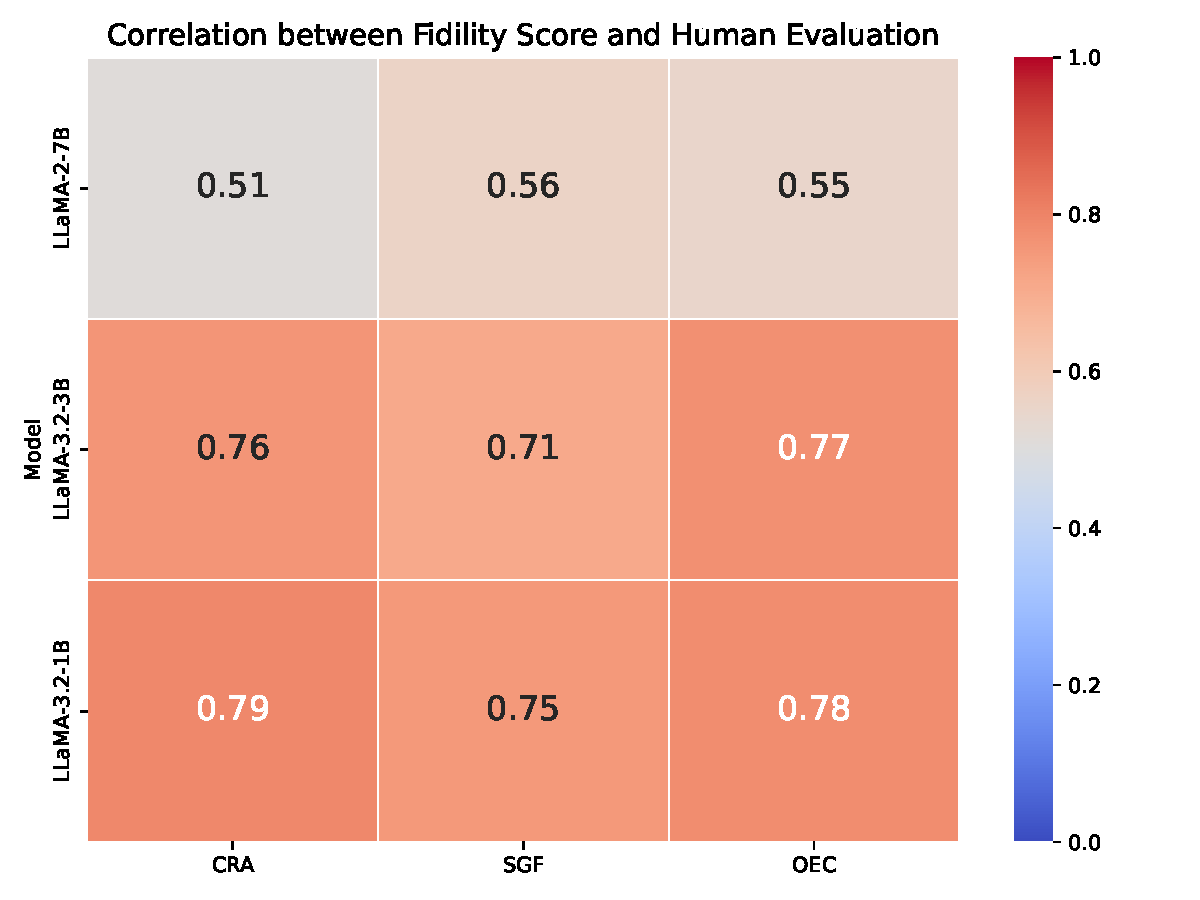
\includegraphics[width=0.9\columnwidth]{correlation_heatmap.pdf}
    \caption{Heatmap visualization of the correlation between the automated round-trip similarity and human evaluation dimensions (CRA, SGF, OEC). Darker colors indicate stronger correlations.}
    \label{fig:correlation_heatmap}
\end{figure}


\paragraph{RQ1 -- Validity of the Automatic Metric.}
To validate the metric independently, we sampled generated outputs \emph{before} applying any selection filter ($\tau_{\text{select}}$), explicitly covering the full fidelity spectrum: early-iteration failures and severe hallucinations (low scores), partially correct outputs (medium), and high-quality generations (high). Human evaluators then \emph{blindly} rated this unfiltered set, ensuring no circular dependency between metric selection and evaluation. We converted A--E ratings to a 5--1 scale. Figure~\ref{fig:correlation_heatmap} shows strong positive correlations (Pearson's $r > 0.5$) between our automatic score $\operatorname{sim}(S,\hat S, \alpha)$ and human ratings for CRA and SGF across this full unfiltered range, validating the metric as an effective, independent, low-cost quality filter. Correlation with OEC was positive but lower, indicating that fidelity scores only partially capture creativity. Inter-annotator agreement (Table~\ref{tab:agreement_tab}) was substantial (87.6\%--89.8\%, Fleiss's $\kappa$ 0.61--0.68), confirming the reliability of human assessments.

\begin{table}[t!]
\centering
\small
\begin{tabular}{lccc}
\toprule
\textbf{Model} & \textbf{Off-the-Shelf} & \textbf{Fine-Tuned} & \textbf{$\Delta$} \\
\midrule
LLaMA2-7B     & 2.70 & 3.32 & +0.62 \\
LLaMA3.2-3B   & 2.30 & 4.02 & +1.72 \\
LLaMA3.2-1B   & 1.94 & 2.70 & +0.76 \\
\bottomrule
\end{tabular}
\caption{Average human ratings comparing off-the-shelf and fine-tuned model variants. Higher scores indicate better performance; $\Delta$ is the improvement of the fine-tuned model over the off-the-shelf counterpart.}
\label{tab:overall_rating}
\end{table}

\paragraph{RQ2 -- Self-Synthetic Fine-Tuning.}
We fine-tuned \texttt{LLaMA-3.2-1B}, \texttt{3.2-3B}, and \texttt{2-7B} to generate KGs (five triples) from paragraphs using only self-generated data. Using our loop (100 cycles), we selected the top-10 high-fidelity texts for each of the 200 training KGs, yielding 2,000 synthetic training samples. Testing was performed on the 50 held-out KG-text pairs (Sec. \ref{sec:eval_data}; examples in Appendix \ref{appendix:examples_training}).
Human annotators rated base vs.\ fine-tuned models on a 5-point scale (converted A--E $\to$ 5--1). Table~\ref{tab:overall_rating} confirms that fine-tuned models consistently outperform base versions. Table~\ref{tab:agreement_tab} shows substantial agreement on the 100 shared items across CRA (89.8\%, $\kappa=0.63$), OEC (88.2\%, $\kappa=0.68$), and SGF (87.6\%, $\kappa=0.61$), confirming assessment reliability. In blinded side-by-side comparisons, annotators strongly preferred the fine-tuned variants (Figure~\ref{fig:preference_counts}).
\begin{figure}[t!]
\centering
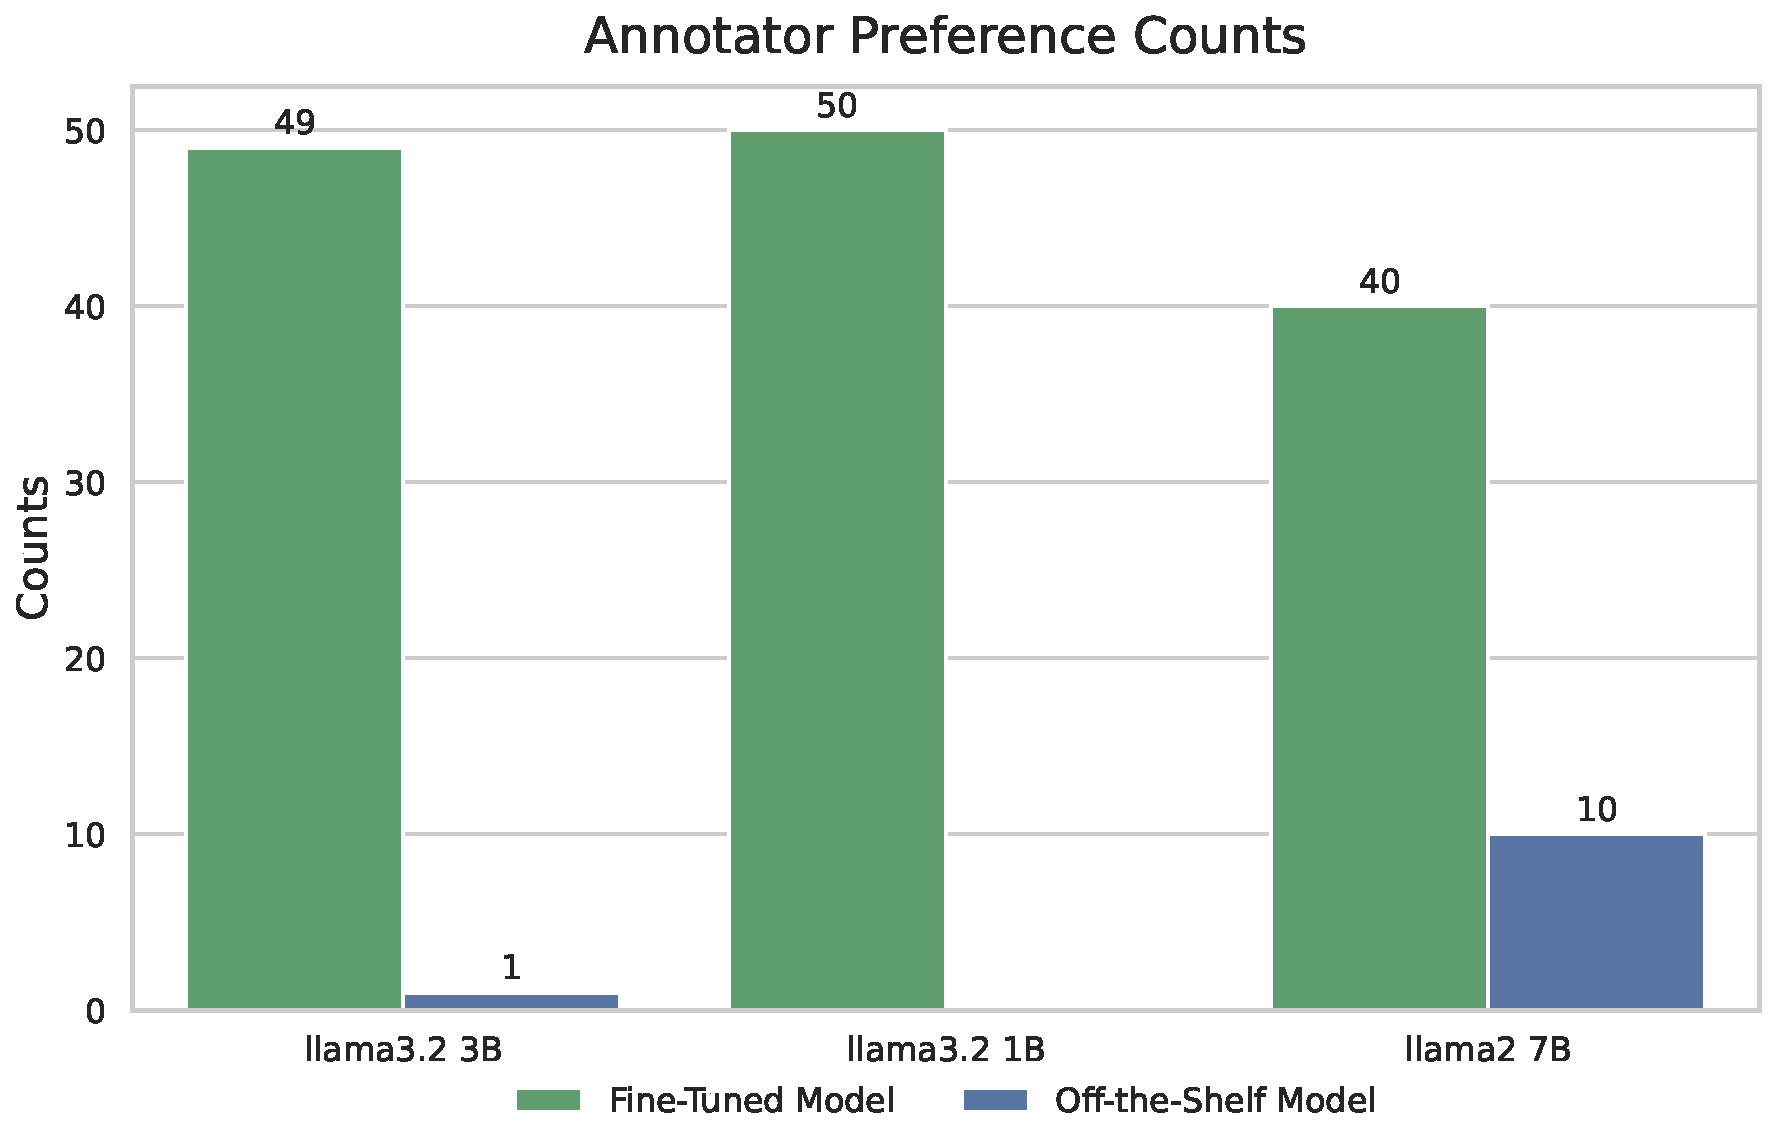
\includegraphics[width=0.9\columnwidth]{perference_counts.pdf}
\caption{Annotator preferences indicating strong favorability towards fine-tuned models compared to off-the-shelf versions.}
\label{fig:preference_counts}
\end{figure}
Automated metrics (BERT F1, ROUGE-L F1, BLEU-4) further corroborate these improvements (Table~\ref{tab:automatic_metrics}). We note that absolute automatic metric values (e.g., BLEU-4 peaking at 0.151) may appear modest; however, this reflects well-documented limitations of n-gram and string-matching metrics when applied to structured extraction tasks rather than model failure. Multiple valid triple formulations exist for the same semantic content (e.g., ``Parthenon $\to$ located\_in $\to$ Athens'' vs.\ ``Parthenon $\to$ city $\to$ Athens''), and minor lexical differences are heavily penalized by these metrics despite semantic equivalence. This is precisely why blinded human evaluation was adopted as our primary standard, where the fine-tuned 3B model achieves a +1.72 point improvement and is overwhelmingly preferred by annotators (49-to-1, Figure~\ref{fig:preference_counts}).\\
The rating distribution in Figure~\ref{fig:rating_distribution} highlights that fine-tuning shifts outputs toward the higher-quality end of the scale. Finally, Figure~\ref{fig:bert_bleu_fraction} demonstrates that performance gains are monotonic with respect to synthetic data volume, with significant jumps appearing even at 25\% data usage.

\begin{table*}[t!]
\centering
\small
\begin{tabular}{lcccccc}
\toprule
Model & \multicolumn{2}{c}{BERTScore F1} & \multicolumn{2}{c}{ROUGE-L F1} & \multicolumn{2}{c}{BLEU-4} \\
& Base & Fine-Tuned & Base & Fine-Tuned & Base & Fine-Tuned \\
\midrule
LLaMA2-7B     & 0.438 & 0.505 & 0.382 & 0.419 & 0.131 & \textbf{0.151} \\
LLaMA3.2-3B   & 0.372 & \textbf{0.514} & 0.409 &\textbf{0.442}  & 0.089 & 0.147 \\
LLaMA3.2-1B   & 0.329 & 0.399 & 0.347 & 0.300 & 0.072 & 0.086 \\
\bottomrule
\end{tabular}
\caption{Comparison of automated evaluation metrics for off-the-shelf (Base) versus fine-tuned variants. Higher scores indicate better performance.}
\label{tab:automatic_metrics}
\end{table*}

\begin{figure*}[ht]
\centering
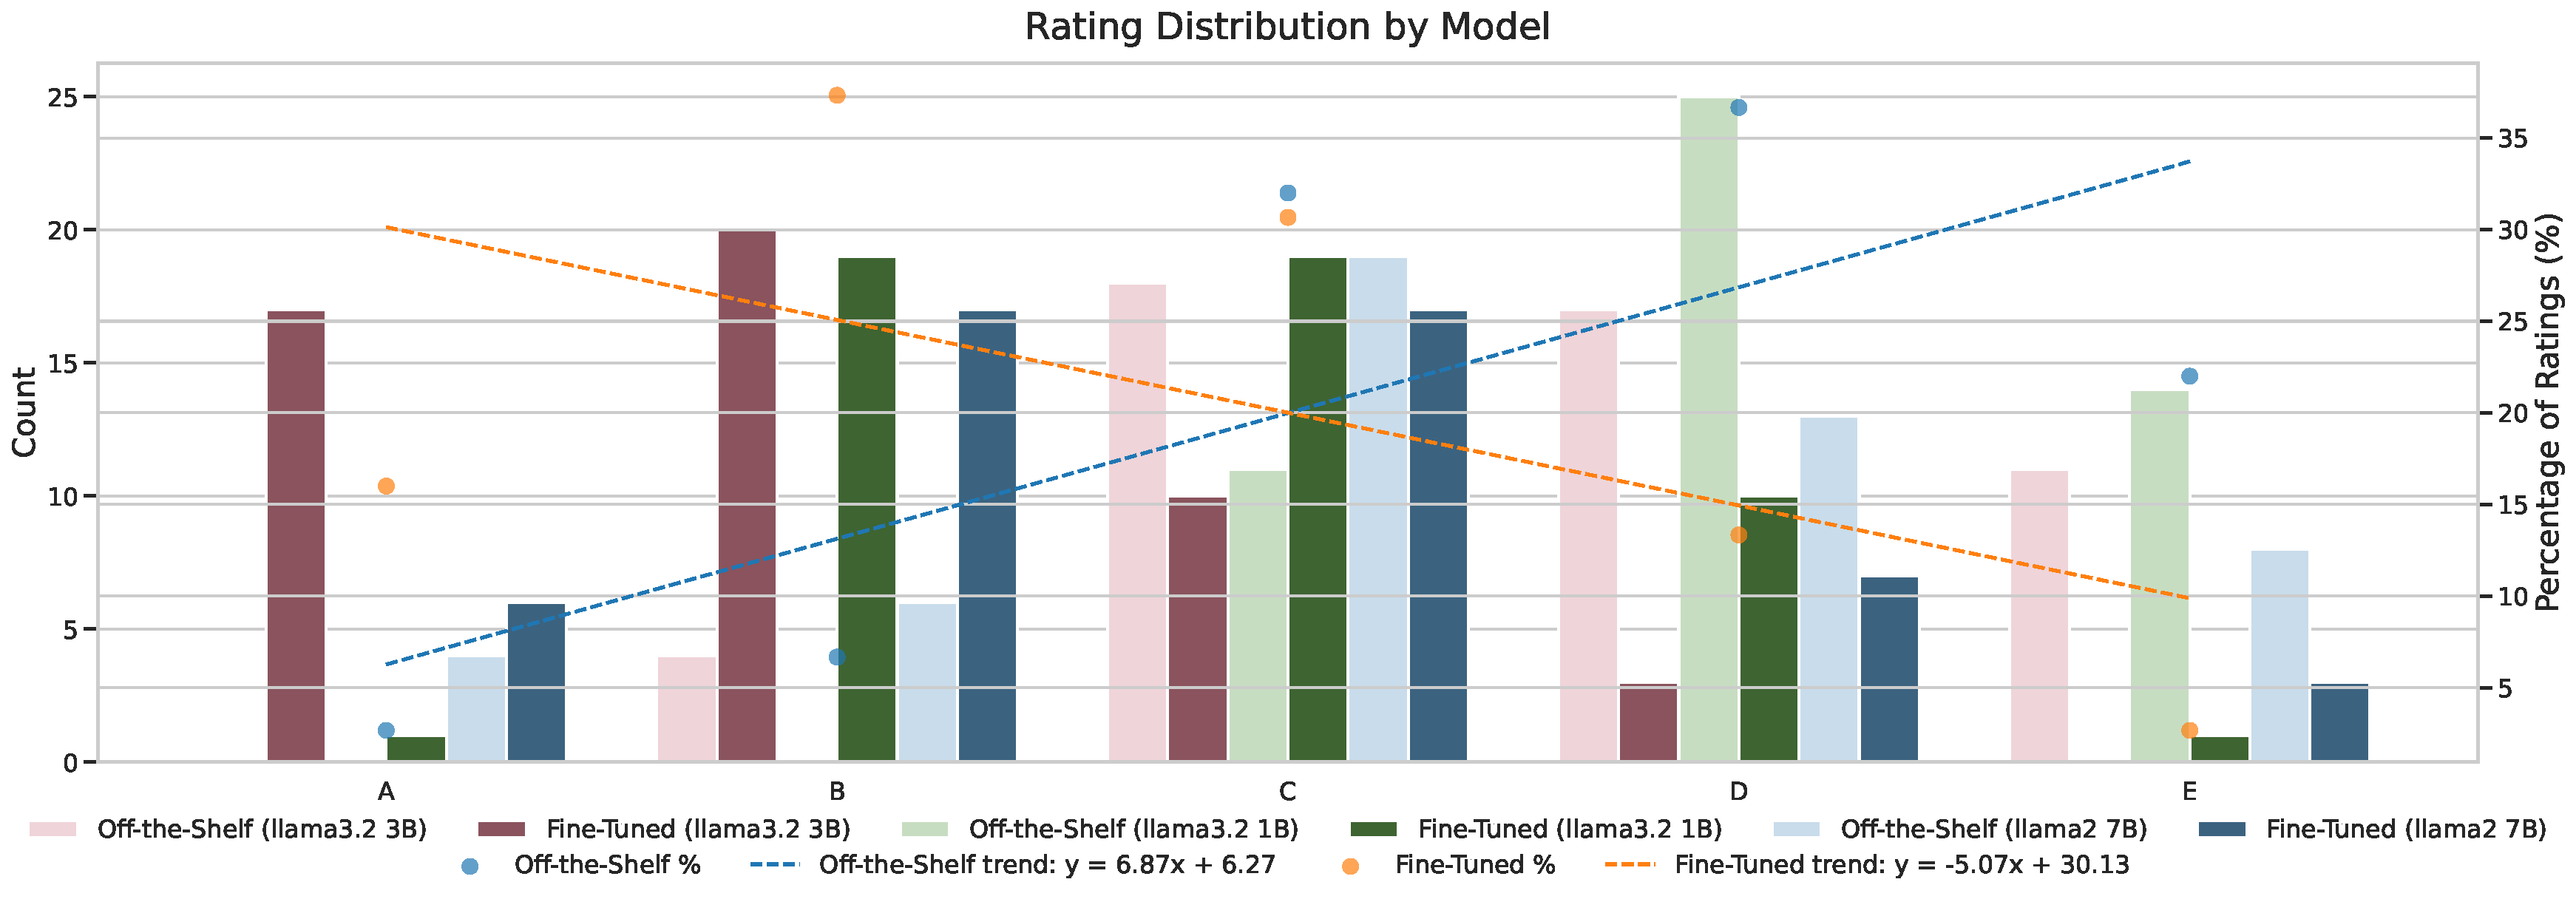
\includegraphics[width=\textwidth]{kg_rating_distribution_legends_swapped.pdf}
\caption{Distribution of annotator ratings (A–E). Darker bars (fine-tuned) dominate the high-quality end (left), while lighter bars (off-the-shelf) concentrate at the low-quality end (right). Dashed trend lines (fine-tuned: $y = -5.07x + 30.13$, off-the-shelf: $y = 6.87x + 6.27$) quantify this divergence.}
\label{fig:rating_distribution}
\end{figure*}


\begin{figure}[h!]
\centering
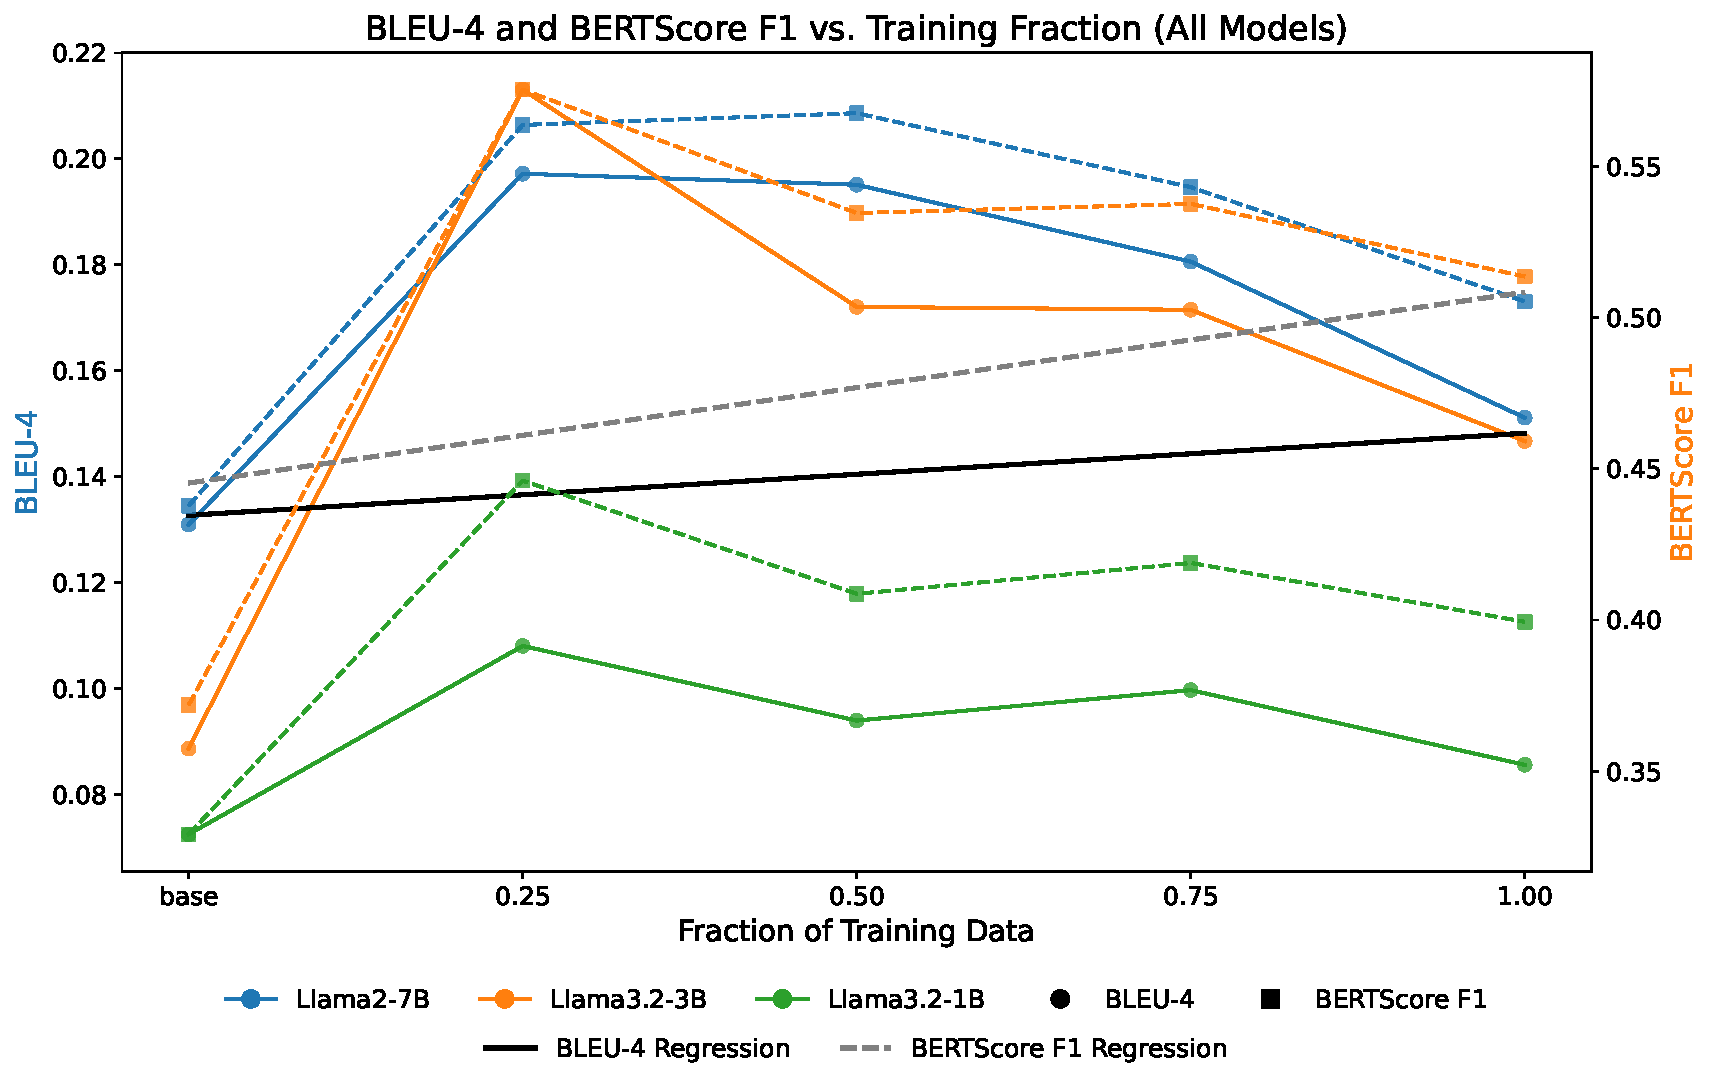
\includegraphics[width=\columnwidth]{bleu_bert_final_connected.pdf}
\caption{BLEU-4 and BERTScore F1 vs.\ Fraction of Training Data. Performance rises steadily from 25\% to 100\%, showing monotonic gains in lexical and semantic quality as synthetic volume increases.}
\label{fig:bert_bleu_fraction}
\end{figure}



\paragraph{Efficiency Ablation.}
To evaluate the impact of data volume, we retrained models using 25\%, 50\%, 75\%, and 100\% of the synthetic dataset, averaging results over three random seeds per fraction. As shown in Figure~\ref{fig:bert_bleu_fraction}, the most significant performance jumps occur at just 25\%, with diminishing returns thereafter. This demonstrates that \emph{quality} drives improvement more than sheer quantity, suggesting that small, high-fidelity datasets can efficiently boost structured knowledge extraction while minimizing resource costs.

\section{Conclusion}

Deploying trustworthy, high-stakes industrial AI requires accurately verbalizing structured enterprise assets. To affordably overcome the ``hallucination bottleneck,'' our \textbf{high-fidelity round-trip pipeline} enforces strict semantic consistency via a self-supervised feedback loop, which experiments validate for industrial deployment:\\
\noindent \textbf{RQ1 (Automated Auditing):} We demonstrated that our automated \textbf{round-trip similarity score} $\operatorname{sim}(S,\hat S, \alpha)$ correlates strongly with expert human judgment ($r > 0.5$). This confirms the metric can serve as a scalable, automated proxy for costly subject-matter expert review.
\noindent \textbf{RQ2 (Cost-Effective Bootstrapping):} We proved that open-weights LLMs can significantly improve their own extraction capabilities using \emph{only} self-generated data. Notably, \texttt{LLaMA3.2-3B} achieved a human-rated quality jump of \textbf{+1.72 points} (on a 5-point scale), demonstrating that expensive proprietary teacher models are not required for high performance.
Crucially, ablation studies revealed that these gains are driven by data \emph{fidelity} rather than volume, with substantial improvements appearing after using only 25\% of the synthetic corpus. This offers a highly efficient path for deploying reliable, KG-grounded AI systems while minimizing compute and labeling overhead. Future work will extend this architecture to complex enterprise formats, such as hierarchical databases and logs.

\section*{Limitations}

While our proposed method demonstrates significant advantages, several limitations merit discussion.

\paragraph{Experimental scope.}
Our experiments use KG triples with five triples per subject. Although the pipeline is representation-agnostic---since similarity evaluation relies on text-to-text semantic comparisons rather than graph-specific heuristics---its practical efficacy on more complex industrial structured data (e.g., deeply nested hierarchical databases, enterprise logs, or irregular schemas with domain-specific long-tail entities) remains to be rigorously evaluated. We note that chunking KGs into 5-triple subgraphs mirrors the localized subgraph retrieval step used in real-world industrial GraphRAG pipelines, which do not feed massive, unchunked graphs to LLMs. Nevertheless, scaling experiments to larger and more complex enterprise KGs is an important direction for future work.

\paragraph{Corpus size.}
Our evaluation corpus of 250 Wikipedia-derived KGs is deliberately small to enable meticulous, triple-by-triple expert human evaluation---a process that is prohibitively expensive to scale, and precisely the bottleneck our pipeline addresses. While our ablation study (Figure~\ref{fig:bert_bleu_fraction}) demonstrates that peak performance is achievable with just 25\% of this data (prioritizing quality over quantity), the generalization to highly domain-specific or low-resource KGs with entities poorly represented in LLM pre-training data remains an open question.

\paragraph{Computational overhead.}
Running the generation loop for $N = 100$ iterations per sample incurs a one-time offline compute cost during synthetic dataset construction. However, this cost is strictly offline; once the fine-tuning dataset is created, model training is fast (e.g., $\sim$15 minutes for the 3B model on our hardware) and the deployed model performs standard single-pass inference with zero additional overhead.

\paragraph{Self-training risks.}
While the structural back-translation step acts as a strong regularizer against factual hallucinations, stylistic biases present in the base model may still propagate through iterative self-training. Future studies should investigate potential saturation points and explore hybrid strategies, such as injecting lightweight expert spot-checks on a small fraction of accepted data before fine-tuning.

\paragraph{Model scale.}
Due to computational constraints, we restricted experiments to models up to 7B parameters. While this allowed clearer observation of quality differences and closer alignment with human judgment, larger models may yield further improvements and should be explored in future work.
%While our proposed method demonstrates significant advantages, limitations remain. Primarily, our experiments were confined to KG triples, and although the methodology is theoretically extensible to other structured forms, its practical efficacy and necessary adaptations remain to be rigorously evaluated.\\
%A limitation is the reliance on 
% predefined 
%automatic metrics,
% and thresholds
%which, although effective in our experiments, might require
%threshold
%task-specific tuning for optimal performance across different domains.
%To address this, we employ human evaluation, however further analysis could be conducted.\\
%Moreover, while our approach successfully employs a model's self-generated data for performance enhancement, further research should investigate potential diminishing returns or saturation points of iterative self-training. \\
% Our experiments focus on rather small language models (up to 7B) to demonstrate that our approach works with such a limited number of parameters thanks to good quality data. However, bigger models could further boost performance.
%Finally, our current evaluation predominantly focuses on semantic fidelity and linguistic quality. A comprehensive exploration of computational cost and efficiency, particularly with larger datasets or more complex structures, 
% remains essential 
%should be investigated for broader applicability.
\section*{Ethics Statement}
LLMs are known to exhibit biases present in their training data and to generate hallucinated content. We use LLMs for the purpose for which they were designed---generating text and triples---and further train them on self-generated content. Therefore, there is a risk of propagating the intrinsic limitations of LLMs.

While our strict structural back-translation step mitigates factual hallucinations, it does not fully address stylistic or representational biases that may be present in the base models. In industrial settings, we recommend treating our pipeline as a ``human-in-the-loop multiplier'': injecting lightweight Subject Matter Expert (SME) spot-checks at the Automated Selection phase (Step 4) on a small fraction of accepted data before fine-tuning. This strategy prevents bias drift while still reducing manual annotation costs by over 90\%.

The data used in this study was solely utilized as a textual corpus derived from publicly available Wikipedia content, and the content should not be interpreted as an endorsement by our team.  
%Addressing potential biases within the data is an area for future research.

% \section*{Acknowledgments}



% Bibliography entries for the entire Anthology, followed by custom entries
%\bibliography{anthology,custom}
% Custom bibliography entries only
\bibliography{custom}


% --------------------  Appendix ---------------------------------
%\clearpage
\appendix
\section{Komodo Dragon Example Materials} \label{appendix:dragon_example}
\subsection{Original Long Texts}

\paragraph{High‑fidelity (raw)}
\begin{quote}
The Komodo Dragon, native to the Indonesian islands, is a formidable creature renowned for its massive size, as it is known as the largest living lizard. This apex predator has evolved to be a stealthy hunter, primarily employing the art of ambush to catch its unsuspecting prey. Its potent venom, delivered through a bite, serves as a deadly deterrent, ensuring that even the most formidable opponents fall prey to its cunning tactics. Despite its impressive stature and formidable abilities, the Komodo Dragon is unfortunately classified as a vulnerable species, necessitating conservation efforts to protect this incredible creature and its dwindling habitat.
\end{quote}

\paragraph{Low‑fidelity (raw)}
\begin{quote}
Deep within the Indonesian archipelago, a majestic creature has long been revered for its awe‑inspiring dominance, the Komondo Dragon, a behemothic reptile whose imposing stature has earned it a revered position in the rich cultural heritage of the region. As the undisputed monarch of its domain, this formidable predator has honed its skills to perfection, utilizing its potent arsenal in calculated precision to subdue its prey, often employing a stealthy ambush tactic that leaves its quarry bewildered and helpless. However, as human encroachment threatens the delicate balance its ecosystem, conservation efforts have become more pressing than ever, ensuring the long‑term survival of this magnificent creature, a poignant reminder that preserving biodiversity is crucial for maintaining the intricate web of life that sustains our planet.
\end{quote}

% -------------------------------------------------------------
% A.2  Zipped Sentences
% -------------------------------------------------------------

\subsection{Zipped Sentences}
The following compressed versions retain only the key facts used in our
quality‑evaluation pipeline:

\begin{description}
  \item[High‑fidelity] The \textbf{Komodo Dragon}, \textbf{native to the Indonesian islands}, is the \textbf{largest living lizard} and an \textbf{apex predator}. It relies on \textbf{ambush tactics} and a \textbf{venomous bite as a deadly deterrent}.
  \item[Low‑fidelity] The \textbf{Komondo Dragon} is \textbf{revered} as the \textbf{monarch of its domain}, famed for \textbf{skills honed to perfection} and a lethal \textbf{arsenal that subdues prey}; many believe its presence keeps the \textbf{ecosystem in balance}.
\end{description}

% -------------------------------------------------------------
% A.3  Extracted Triples  (wide)
% -------------------------------------------------------------

\subsection{Extracted Triples}
Table~\ref{tab:triples} lists the subject–predicate–object triples
identified by the information‑extraction step for each long text.

\begin{table*}[htbp]
  \centering
  \caption{Triples extracted from each text.}
  \label{tab:triples}
  \begin{tabular}{@{}lp{14cm}@{}}
    \toprule
    \textbf{Source} & \textbf{Triple (subject $\to$ relation $\to$ object)} \\
    \midrule
    High‑fid.& (Komodo Dragon $\to$ native\_to $\to$ Indonesian islands) \\
             & (Komodo Dragon $\to$ known\_as $\to$ largest living lizard) \\
             & (Komodo Dragon $\to$ type $\to$ apex predator) \\
             & (Komodo Dragon $\to$ employed $\to$ art of ambush) \\
             & (Komodo Dragon $\to$ venom $\to$ deadly deterrent) \\
    \addlinespace[4pt]
    Low‑fid.& (Komondo Dragon $\to$ revered $\to$ position) \\
             & (Komondo Dragon $\to$ monarch $\to$ domain) \\
             & (Komondo Dragon $\to$ skills $\to$ perfection) \\
             & (Komodo Dragon $\to$ arsenal $\to$ prey) \\
             & (Komodo Dragon $\to$ ecosystem $\to$ balance) \\
    \bottomrule
  \end{tabular}
\end{table*}

% -------------------------------------------------------------
% A.4  Alignment Tables  (both wide)
% -------------------------------------------------------------

\subsection{Alignment Tables}
To demonstrate how the compression preserves--or distorts--meaning,
Tables~\ref{tab:long2zip} and~\ref{tab:tri2zip} provide two complementary
views of the alignment.



\begin{table*}[htbp]
  \centering
  \caption{Alignment of key phrases from the long texts to the zipped sentences. Ellipses (\ldots) indicate intervening words.}
  \label{tab:long2zip}
  \begin{tabular}{@{}lp{6.2cm}p{6.2cm}@{}}
    \toprule
    \textbf{Fidelity} & \textbf{Excerpt in Long Text} & \textbf{Corresponding Zipped Phrase} \\
    \midrule
    High & native to the Indonesian islands & native to the Indonesian islands \\
         & largest living lizard & largest living lizard \\
         & This apex predator & apex predator \\
         & employing the art of ambush & ambush tactics \\
         & venom\ldots{} deadly deterrent & venomous bite as a deadly deterrent \\
    \addlinespace[3pt]
    Low  & revered\ldots{} revered position & revered \dots{} position \\
         & undisputed monarch of its domain & monarch of its domain \\
         & skills to perfection & skills honed to perfection \\
         & arsenal\ldots{} subdue its prey & arsenal that subdues prey \\
         & delicate balance its ecosystem & ecosystem in balance \\
    \bottomrule
  \end{tabular}
\end{table*}


\subsubsection{
%A.4.2 
Triple $\rightarrow$ Zipped Phrase}

Table \ref{tab:tri2zip} shows alignment of extracted triples to phrases in the zipped sentences.

\begin{table*}[htbp!]
  \centering
  \caption{Alignment of extracted triples to phrases in the zipped sentences.}
  \label{tab:tri2zip}
  \begin{tabular}{@{}lp{6.2cm}p{6.2cm}@{}}
    \toprule
    \textbf{Fidelity} & \textbf{Triple Predicate} & \textbf{Phrase in Zipped Sentence} \\
    \midrule
    High & native\_to   & native to the Indonesian islands \\
         & known\_as    & largest living lizard \\
         & type         & apex predator \\
         & employed     & ambush tactics \\
         & venom        & venomous bite as a deadly deterrent \\
    \addlinespace[3pt]
    Low  & revered      & revered \dots{} position \\
         & monarch      & monarch of its domain \\
         & skills       & skills honed to perfection \\
         & arsenal      & arsenal that subdues prey \\
         & ecosystem    & ecosystem in balance \\
    \bottomrule
  \end{tabular}
\end{table*}

% ---------- A.4  Explanatory Note ----------
\subsection{Explanatory Note}

Similarity is computed by comparing triples in each reconstructed KG
($\hat S_1$, $\hat S_2$) with those in the original KG $S$ using an
similarity metric over complete \emph{(subject, relation, object)} units.
Because all five triples are recovered from the high-fidelity text, its
score approaches 0.8 .  
The low-fidelity text drifts into mythic language and misspells
“Komodo,” so only superficial overlaps remain, producing the lower score
of 0.45.


\section{Reproducibility}
\label{appendix:reproducibility}

\subsection{Round–Trip Generation Loop Parameters. }
\label{ssec:loop-config}
Algorithm~\ref{alg:loop} runs for iterative text generation cycles (\( N = 100 \)) using the hyperparameters optimized on a development set: initial decoding temperature \( t_0 = 0.8 \), temperature increment \( \Delta t = 0.9 \), initial top-p \( p_0 = 0.8 \), top-p increment \( \Delta p = 0.5 \), with similarity thresholds \( \tau_{\text{low}} = 0.5 \) and \( \tau_{\text{high}} = 0.9 \). We used the ROUGE-L F-measure for evaluating textual similarity ($Sim_{Lex}$) and the e5-mistral-large model for computing cosine embedding similarity.
%%%%%%%%%%%%%%%%%%%%%%%%%%%%%%%%%%%%%%%%%%%%%%%%%%%%%%%%%%%%%%%%%%%%%%%
\subsection{Prompts}
\label{ssec:prompts}
%%%%%%%%%%%%%%%%%%%%%%%%%%%%%%%%%%%%%%%%%%%%%%%%%%%%%%%%%%%%%%%%%%%%%%%

The exact prompt templates used in both directions are reproduced
below (placeholders \texttt{\{KG\}}, \texttt{\{REF\}},
\texttt{\{PARAGRAPH\}} are filled at runtime).  
Templates follow the instruction\(+\)input schema of
\citet{liu2024best}.  The reference paragraph appears only on even
iterations to promote lexical diversity.

\vspace{0.3em}
\noindent\textbf{KG $\rightarrow$ Text (first pass)}
\begin{lstlisting}[style=prompt]
System: You are a helpful assistant skilled in generating
        descriptive paragraphs from knowledge-graph triples.
User  : Using the following knowledge-graph triples, craft a
        detailed paragraph of at least 70 words that elaborates on
        the information provided. Return only the generated text.
        {KG}
\end{lstlisting}

\noindent\textbf{KG $\rightarrow$ Text (subsequent passes)}
\begin{lstlisting}[style=prompt]
System: You are a creative assistant skilled in crafting original
        content based on provided data.
User  : Using the knowledge-graph triples provided below, write a
        clear and original paragraph of at least 70 words. The
        paragraph must begin with the subject of the triples and
        must include all information accurately from the triples
        nothing should be left out or misrepresented.
        While the paragraph should differ from the reference, it
        need not be drastically different. Return only the paragraph.

Reference Paragraph:
{REF}

Knowledge-Graph Triples:
{KG}
\end{lstlisting}

\noindent\textbf{Text $\rightarrow$ KG}
\begin{lstlisting}[style=prompt]
System: You are a helpful assistant specialised in extracting
        structured data.
User  : Extract exactly five knowledge-graph triples from the text
        below in the form (Entity -> Relation -> Object). Return only
        the extracted triples.

TEXT:
{PARAGRAPH}
\end{lstlisting}


\subsection{Training Configuration}
\label{ssec:training}

All self-fine-tuning experiments were conducted with
\texttt{Transformers v4.41} and \texttt{DeepSpeed 0.14} in ZeRO-2
mode on four NVIDIA RTX A6000 GPUs (48 GB each).
Input sequences were truncated or padded to a maximum of 512 tokens,
and each model was trained for three full epochs.
Optimisation used \texttt{bf16} precision, an initial learning rate of
\(1\times10^{-4}\) that followed a cosine decay schedule, and a
per-device batch size of four; two-step gradient accumulation yielded
an effective batch size of 16.
Gradient checkpointing and FlashAttention-2 were enabled to keep the
memory footprint is low and throughput is high.
Parameter-efficient tuning relied on LoRA: $rank=16$ adapters with
\(\alpha=32\) and a dropout of $0.1$ were attached to all projections
layers (\textit{q\_proj}, \textit{k\_proj}, \textit{v\_proj},
\textit{o\_proj}, \textit{down\_proj}, \textit{up\_proj},
\textit{gate\_proj}) as well as the embedding matrix and the language-model head.
With this configuration the entire three-epoch run over the 2,000
self-synthetic training pairs completed in roughly 135 minutes,
peaking at about 48 GB of GPU memory per card.\\
 For the \texttt{LLaMA-3.2-1B} model, training with full dataset required approximately 8 minutes with an average GPU utilization of 24.8\%. The \texttt{LLaMA-3.2-3B} model completed training in 15 minutes with a utilization of 27.01\%, while the \texttt{LLaMA-2-7B} model required 22 minutes and exhibited an average GPU utilization of 36.7\%. 
\paragraph{Inference Hyperparameter:}
Inference was performed using the following parameters: temperature set to 0.7, top-$k$ of 50, top-$p$ of 0.9, and a repetition penalty of 1.1.
\subsection{Hyperparameter Selection}\label{appendix:params_selection}
Hyperparameters were determined empirically through systematic experimentation and tuning on a held-out development set. Specifically, we employed a grid-search strategy to optimize the decoding temperature and top-$p$ sampling thresholds, evaluating their impact on semantic fidelity measured via our defined round-trip similarity. The final hyperparameter values were selected to achieve a balance between linguistic diversity and factual accuracy, ensuring the generation of high-quality synthetic text without compromising semantic consistency.
\section{Annotation Guidelines}
\label{appendix:guidelines}

\subsection{Annotation Guidelines for RQ1}
\label{appendix:guidelines1}

Annotators were instructed to follow these specific guidelines for evaluating each paragraph:\\

\noindent\textbf{Content \& Relation Accuracy (CRA):}
\begin{itemize}
\item[A:] Perfect accuracy, no omissions or factual errors.
\item[B:] Minor omissions or inaccuracies that do not distort meaning significantly.
\item[C:] Moderate omissions or inaccuracies affecting some details.
\item[D:] Major inaccuracies or frequent omissions significantly distorting meaning.
\item[E:] Severe inaccuracies or entirely incorrect representation of facts.
\end{itemize}

\noindent\textbf{Structure, Grammar \& Fluency (SGF):}
\begin{itemize}
\item[A:] Completely fluent and grammatically correct; excellent readability and coherence.
\item[B:] Mostly fluent with minor grammar or structural issues; good coherence.
\item[C:] Moderate grammar or structure issues; readability somewhat compromised.
\item[D:] Frequent grammatical or structural errors significantly affecting readability.
\item[E:] Severely flawed grammar and structure; very poor readability and coherence.
\end{itemize}

\noindent\textbf{Originality, Engagement \& Creativity (OEC):}
\begin{itemize}
\item[A:] Highly original, engaging, and creative; text feels natural and varied.
\item[B:] Good creativity and originality; engaging but somewhat predictable.
\item[C:] Moderate originality; limited creativity; somewhat repetitive.
\item[D:] Minimal originality; repetitive phrasing and low engagement.
\item[E:] Completely repetitive or uncreative; extremely limited engagement and originality.
\end{itemize}





\subsection{Annotation Guidelines for RQ2}\label{appendix:guidelines2}

Annotators followed this detailed guideline for rating generated KGs on a scale from A (excellent) to E (unacceptable):\\

\noindent\textbf{A – Excellent}
\begin{itemize}
\item Exactly 5 triples, formatted as (Subject -> Predicate -> Object), no extraneous text.
\item All triples capture key facts accurately and reflect the original text precisely.
\item Triples are logically structured, semantically clear, and insightful.
\end{itemize}

\noindent\textbf{B – Good}
\begin{itemize}
\item Generally 5 correctly formatted triples; minor formatting issues allowed.
\item Most triples accurately represent the text; minor omissions or slight inaccuracies acceptable.
\item Triples are mostly clear and logically structured; slight clarity improvements possible.
\end{itemize}

\noindent\textbf{C – Satisfactory}
\begin{itemize}
\item Roughly 5 triples; slight deviations or minor formatting issues.
\item Main ideas captured; some details missing or slightly misrepresented.
\item Valid triples, but some have ambiguous or weakly defined relationships.
\end{itemize}

\noindent\textbf{D – Poor}
\begin{itemize}
\item Noticeable deviations from 5-triple expectation or significant formatting issues.
\item Several key aspects misinterpreted or omitted.
\item Many triples vague, unclear, or incorrectly structured.
\end{itemize}

\noindent\textbf{E – Unacceptable}
\begin{itemize}
\item Incorrect number or badly formatted triples.
\item Triples irrelevant, randomly generated, or completely off-topic.
\item Triples are incoherent, incomplete, contradictory, or nonsensical.
\end{itemize}

%\appendix
\section{Example Knowledge Graphs}
\label{sec:appendix-kgs}
\subsection{Knowledge Graph Examples}\label{sec:appendix-kgs1}
Each KG is represented as a list of factual triples in the
form \mbox{(head $\rightarrow$ relation $\rightarrow$ tail)}.  
Here are five diverse topics that are representative of the dataset used in
our experiments. 

\begin{itemize}[leftmargin=*]  % remove the bracket if you don't load enumitem
\item \textbf{African Elephant}
  \begin{itemize}[leftmargin=1em]
  \item (African Elephant $\rightarrow$ is native to $\rightarrow$ Sub-Saharan Africa)
  \item (African Elephant $\rightarrow$ has $\rightarrow$ large tusks)
  \item (African Elephant $\rightarrow$ is classified as $\rightarrow$ vulnerable species)
  \item (African Elephant $\rightarrow$ possesses $\rightarrow$ high intelligence)
  \item (African Elephant $\rightarrow$ lives in $\rightarrow$ herds)
  \end{itemize}

\item \textbf{Apollo 11 Moon Landing}
  \begin{itemize}[leftmargin=1em]
  \item (Apollo 11 Moon Landing $\rightarrow$ occurred\_on $\rightarrow$ July 20, 1969)
  \item (Apollo 11 Moon Landing $\rightarrow$ mission\_commander $\rightarrow$ Neil Armstrong)
  \item (Apollo 11 Moon Landing $\rightarrow$ included\_astronauts $\rightarrow$ Neil Armstrong, Buzz Aldrin, Michael Collins)
  \item (Apollo 11 Moon Landing $\rightarrow$ first\_moonwalker $\rightarrow$ Neil Armstrong)
  \item (Apollo 11 Moon Landing $\rightarrow$ spacecraft\_used $\rightarrow$ Apollo 11)
  \end{itemize}

\item \textbf{Quantum Mechanics}
  \begin{itemize}[leftmargin=1em]
  \item (Quantum Mechanics $\rightarrow$ describes behavior of $\rightarrow$ atomic-scale particles)
  \item (Quantum Mechanics $\rightarrow$ introduces concept of $\rightarrow$ wave-particle duality)
  \item (Quantum Mechanics $\rightarrow$ is characterized by $\rightarrow$ uncertainty principle)
  \item (Quantum Mechanics $\rightarrow$ was pioneered by $\rightarrow$ Max Planck)
  \item (Quantum Mechanics $\rightarrow$ forms basis for $\rightarrow$ quantum computing)
  \end{itemize}

\item \textbf{Climate Change}
  \begin{itemize}[leftmargin=1em]
  \item (Climate Change $\rightarrow$ is defined as $\rightarrow$ long-term alterations in average temperature and weather patterns)
  \item (Climate Change $\rightarrow$ is primarily caused by $\rightarrow$ human activities such as burning fossil fuels)
  \item (Climate Change $\rightarrow$ results in $\rightarrow$ rising global temperatures)
  \item (Climate Change $\rightarrow$ leads to $\rightarrow$ melting polar ice caps)
  \item (Climate Change $\rightarrow$ affects $\rightarrow$ ecosystems and biodiversity)
  \end{itemize}

\item \textbf{Internet}
  \begin{itemize}[leftmargin=1em]
  \item (Internet $\rightarrow$ invented\_by $\rightarrow$ ARPANET project)
  \item (Internet $\rightarrow$ introduced\_in\_year $\rightarrow$ 1969)
  \item (Internet $\rightarrow$ is\_based\_on\_protocol $\rightarrow$ TCP/IP)
  \item (Internet $\rightarrow$ enabled\_services $\rightarrow$ Email)
  \item (Internet $\rightarrow$ has\_main\_feature $\rightarrow$ global connectivity)
  \end{itemize}
\end{itemize}

\subsection{Paired Text--KG Examples}
\label{sec:appendix-kgs2}

The following examples present a short descriptive paragraph \emph{paired} with its corresponding knowledge-graph (KG) triples.  The format illustrates how free text can be grounded in a structured representation.

\paragraph{\textit{The Alhambra}}
The Alhambra, located in Granada, Spain, is a stunning example of Islamic architecture.  Built by the Nasrid dynasty during the 13\textsuperscript{th}–14\textsuperscript{th} centuries, its intricate arabesque carvings, courtyards, and reflecting pools embody Moorish artistic ideals.  Its cultural importance and exceptional state of preservation have earned it recognition as a UNESCO~World~Heritage~Site.

\textbf{Knowledge Graph}
\begin{itemize}[leftmargin=1em]
\item (The Alhambra $\rightarrow$ located in $\rightarrow$ Granada, Spain)
\item (The Alhambra $\rightarrow$ built by $\rightarrow$ Nasrid dynasty)
\item (The Alhambra $\rightarrow$ architectural style $\rightarrow$ Islamic architecture)
\item (The Alhambra $\rightarrow$ recognized as $\rightarrow$ UNESCO World Heritage Site)
\item (The Alhambra $\rightarrow$ famous for $\rightarrow$ intricate decorative designs)
\end{itemize}

\paragraph{\textit{The Parthenon}}
The Parthenon, a masterpiece of Classical Greek architecture, crowns the Acropolis in Athens.  Dedicated to the goddess Athena and completed in the 5\textsuperscript{th}~century~BCE, it exemplifies the Doric order and has influenced Western architecture for millennia.  Despite damage over the ages, the Parthenon remains a powerful symbol of ancient Greek artistry.

\textbf{Knowledge Graph}
\begin{itemize}[leftmargin=1em]
\item (The Parthenon $\rightarrow$ located in $\rightarrow$ Athens, Greece)
\item (The Parthenon $\rightarrow$ dedicated to $\rightarrow$ Goddess Athena)
\item (The Parthenon $\rightarrow$ built during $\rightarrow$ 5th century BCE)
\item (The Parthenon $\rightarrow$ architectural style $\rightarrow$ Classical Greek architecture)
\item (The Parthenon $\rightarrow$ part of $\rightarrow$ the Acropolis of Athens)
\end{itemize}

\paragraph{\textit{The Suez Canal}}
The Suez Canal, in Egypt, is a vital 193\,km waterway that links the Mediterranean and Red Seas, allowing vessels to avoid the longer route around the Cape of Good Hope.  Opened in 1869 and engineered under Ferdinand~de~Lesseps, it remains one of the world’s busiest shipping lanes and is administered by the Suez Canal Authority.

\textbf{Knowledge Graph}
\begin{itemize}[leftmargin=1em]
\item (The Suez Canal $\rightarrow$ connects $\rightarrow$ Mediterranean Sea and Red Sea)
\item (The Suez Canal $\rightarrow$ opened in $\rightarrow$ 1869)
\item (The Suez Canal $\rightarrow$ located in $\rightarrow$ Egypt)
\item (The Suez Canal $\rightarrow$ managed by $\rightarrow$ Suez Canal Authority)
\item (The Suez Canal $\rightarrow$ architect $\rightarrow$ Ferdinand de Lesseps)
\end{itemize}

\paragraph{\textit{The Harlem Renaissance}}
The Harlem Renaissance was a vibrant African-American cultural movement during the 1920s and 1930s, centred in Harlem, New York City.  Writers such as Langston Hughes and Zora Neale Hurston, along with musicians, painters, and activists, celebrated Black life and challenged racial prejudice, laying intellectual groundwork for the later Civil Rights Movement.

\textbf{Knowledge Graph}
\begin{itemize}[leftmargin=1em]
\item (The Harlem Renaissance $\rightarrow$ occurred during $\rightarrow$ 1920s and 1930s)
\item (The Harlem Renaissance $\rightarrow$ centered in $\rightarrow$ Harlem, New York City)
\item (The Harlem Renaissance $\rightarrow$ cultural focus $\rightarrow$ African-American literature and arts)
\item (The Harlem Renaissance $\rightarrow$ notable figure $\rightarrow$ Langston Hughes)
\item (The Harlem Renaissance $\rightarrow$ influenced $\rightarrow$ Civil Rights Movement)
\end{itemize}

\paragraph{\textit{Marie Antoinette}}
Marie Antoinette, born in Vienna in 1755, became Queen of France after her marriage to King Louis XVI.  Her lavish lifestyle and perceived indifference to the plight of commoners contributed to revolutionary fervour.  Arrested during the French Revolution, she was executed by guillotine in 1793, becoming an enduring, controversial historical figure.

\textbf{Knowledge Graph}
\begin{itemize}[leftmargin=1em]
\item (Marie Antoinette $\rightarrow$ born in $\rightarrow$ Vienna, Austria)
\item (Marie Antoinette $\rightarrow$ title held $\rightarrow$ Queen of France)
\item (Marie Antoinette $\rightarrow$ married to $\rightarrow$ King Louis XVI)
\item (Marie Antoinette $\rightarrow$ executed by $\rightarrow$ guillotine)
\item (Marie Antoinette $\rightarrow$ died during $\rightarrow$ French Revolution)
\end{itemize}



\section{Illustrative Extraction Examples Before \& After Fine-Tuning} \label{appendix:examples_training}

\textbf{Examples Before \& After Fine-Tuning}
This appendix presents illustrative examples from each model before and after fine-tuning. The tables below (\ref{tab:parthenon}--\ref{tab:waterloo}) show the extracted KG triples, allowing a direct comparison of model outputs. For each passage we list the knowledge–graph (KG) triples produced by the \emph{Off-the-shelf} model and the \emph{expert-trained} model in {separate
tables.
% ------------------------- Appendix -----------------------

% ----------------------------------------------------------- %
\subsection{Llama-3.2 3B}

\paragraph{Example 1. Parthenon}
\begin{quote}\small
\textit{The Parthenon, a stunning example of Classical Greek architecture, dominates the
Acropolis of Athens. Built in the 5th century BCE and dedicated to the goddess Athena, it
stands as a lasting testament to the artistic and architectural achievements of ancient
Greece.} 
\end{quote}
\noindent\textbf{See Table~\ref{tab:parthenon}.}

\begin{table*}[h]
\centering\small
\caption{KG triples for Example 1 (Parthenon).}\label{tab:parthenon}
\begin{tabular}{@{}p{.17\textwidth}p{.76\textwidth}@{}}
\textbf{Model} & \textbf{Triples}\\\hline
Off-the-shelf &
\ttfamily(Parthenon $\to$ located\_in $\to$ Acropolis\_of\_Athens);\,
(Parthenon $\to$ city $\to$ Athens);\,
(Parthenon $\to$ dedicated\_to $\to$ Goddess\_Athena);\,
(Parthenon $\to$ built\_in $\to$ 5th\_century\_BCE)
\\
Expert-trained &
\ttfamily(Parthenon $\to$ is located in $\to$ Athens, Greece);\,
(Parthenon $\to$ was built in $\to$ the 5th century BC);\,
(Parthenon $\to$ is a landmark of $\to$ Classical Greek architecture);\,
(Parthenon $\to$ is dedicated to $\to$ Goddess Athena);\,
(Parthenon $\to$ is part of $\to$ the Acropolis)
\end{tabular}
\end{table*}

\paragraph{Example 2. Acropolis of Athens}
\begin{quote}\small
\textit{The Acropolis of Athens, perched on a rocky hill above the city, was largely
completed in the 5th century BC. It is a powerful symbol of ancient Greek civilisation and
is today recognised by UNESCO as a World Heritage Site.}
\end{quote}
\noindent\textbf{See Table~\ref{tab:acropolis}.}
\begin{table*}[h]
\centering\small
\caption{KG triples for Example 2 (Acropolis of Athens).}\label{tab:acropolis}
\begin{tabular}{@{}p{.17\textwidth}p{.76\textwidth}@{}}
\textbf{Model} & \textbf{Triples}\\\hline
Off-the-shelf &
\ttfamily(Acropolis $\to$ of $\to$ Athens);\,
(Acropolis $\to$ is $\to$ historic citadel);\,
(Acropolis $\to$ dedicated $\to$ Athena);\,
(Acropolis $\to$ symbol $\to$ ancient Greek civilisation);\,
(Acropolis $\to$ recognised $\to$ UNESCO World Heritage Site)
\\
Expert-trained &
\ttfamily(Acropolis of Athens $\to$ is located in $\to$ Athens, Greece);\,
(Acropolis of Athens $\to$ was built in $\to$ the 5th century BC);\,
(Acropolis of Athens $\to$ is famous for $\to$ the Parthenon);\,
(Acropolis of Athens $\to$ was dedicated to $\to$ goddess Athena);\,
(Acropolis of Athens $\to$ is recognised as $\to$ a UNESCO World Heritage Site)
\end{tabular}
\end{table*}

% ----------------------------------------------------------- %
\subsection{Llama-2 7B}

\paragraph{Example 1. Anne Frank}
\begin{quote}\small
\textit{Anne Frank, born in Frankfurt, Germany, became widely known for the diary she kept
while hiding from the Nazis in Amsterdam. Tragically, she died in 1945 at the
Bergen-Belsen concentration camp. Her diary has been translated into numerous languages and
remains a powerful testament to hope and resilience.}
\end{quote}
\noindent\textbf{See Table~\ref{tab:anne}.}
\begin{table*}[h]
\centering\small
\caption{KG triples for Example 1 (Anne Frank).}\label{tab:anne}
\begin{tabular}{@{}p{.17\textwidth}p{.76\textwidth}@{}}
\textbf{Model} & \textbf{Triples}\\\hline
Off-the-shelf &
\ttfamily(Anne Frank $\to$ born in $\to$ Germany);\,
(Anne Frank $\to$ wrote $\to$ a diary);\,
(Anne Frank $\to$ hid from $\to$ Nazis);\,
(Anne Frank $\to$ died in $\to$ concentration camp);\,
(Diary $\to$ offers $\to$ glimpse of life)
\\
Expert-trained &
\ttfamily(Anne Frank $\to$ born in $\to$ Frankfurt, Germany);\,
(Anne Frank $\to$ authored $\to$ “The Diary of Anne Frank”);\,
(Anne Frank $\to$ hid in $\to$ Amsterdam);\,
(Anne Frank $\to$ died at $\to$ Bergen-Belsen);\,
(Diary of Anne Frank $\to$ translated into $\to$ many languages)
\end{tabular}
\end{table*}

\paragraph{Example 2. Human Genome Project}
\begin{quote}\small
\textit{The Human Genome Project, initiated in 1990 and completed in 2003, set out to
map and understand every human gene. Led by Francis Collins and coordinated by the U.S.
Department of Energy and the National Institutes of Health, it laid the foundation for
major advances in genetics and medicine.}
\end{quote}
\noindent\textbf{See Table~\ref{tab:hgp}.}
\begin{table*}[h]
\centering\small
\caption{KG triples for Example 2 (Human Genome Project).}\label{tab:hgp}
\begin{tabular}{@{}p{.17\textwidth}p{.76\textwidth}@{}}
\textbf{Model} & \textbf{Triples}\\\hline
Off-the-shelf &
\ttfamily(Human Genome Project $\to$ initiated $\to$ 1990);\,
(Human Genome Project $\to$ goal $\to$ map human genes);\,
(Francis Collins $\to$ led $\to$ project);\,
(DOE \& NIH $\to$ coordinated $\to$ project);\,
(Project $\to$ foundation for $\to$ genomics)
\\
Expert-trained &
\ttfamily(Human Genome Project $\to$ began in $\to$ 1990);\,
(Human Genome Project $\to$ completed in $\to$ 2003);\,
(Human Genome Project $\to$ coordinated by $\to$ NIH);\,
(Human Genome Project $\to$ led by $\to$ Francis Collins);\,
(Human Genome Project $\to$ enabled $\to$ personalised medicine)
\end{tabular}
\end{table*}

% ----------------------------------------------------------- %
\subsection{Llama-3.2 1B}

\paragraph{Example 1. Euro}
\begin{quote}\small
\textit{The Euro (€) was introduced in 1999 as the official currency of 11 European Union
member states. The European Central Bank oversees its monetary policy across the Eurozone.}
\end{quote}
\noindent\textbf{See Table~\ref{tab:euro}.}

\begin{table*}[h]
\centering\small
\caption{KG triples for Example 1 (Euro).}\label{tab:euro}
\begin{tabular}{@{}p{.17\textwidth}p{.76\textwidth}@{}}
\textbf{Model} & \textbf{Triples}\\\hline
Off-the-shelf &
\ttfamily(Euro $\to$ introduced $\to$ EU member states);\,
(Euro $\to$ managed by $\to$ European Central Bank);\,
(Euro $\to$ replaced $\to$ national currencies);\,
(Euro $\to$ managed $\to$ monetary policy);\,
(Euro $\to$ managed in $\to$ Eurozone)
\\
Expert-trained &
\ttfamily(Euro $\to$ is the currency used by $\to$ EU members);\,
(Euro $\to$ introduced\_in $\to$ 1999);\,
(Euro $\to$ is administered by $\to$ European Central Bank);\,
(Euro $\to$ replaced $\to$ Deutsche Mark);\,
(Euro $\to$ promotes $\to$ economic integration)
\end{tabular}
\end{table*}

\paragraph{Example 2. Battle of Waterloo}
\begin{quote}\small
\textit{The Battle of Waterloo, fought on 18 June 1815 near Waterloo in present-day Belgium,
marked the final defeat of Napoleon Bonaparte in the Napoleonic Wars. Among the key
commanders was Arthur Wellesley, the Duke of Wellington.}
\end{quote}
\noindent\textbf{See Table~\ref{tab:waterloo}.}
\begin{table*}[h]
\centering\small
\caption{KG triples for Example 2 (Battle of Waterloo).}\label{tab:waterloo}
\begin{tabular}{@{}p{.17\textwidth}p{.76\textwidth}@{}}
\textbf{Model} & \textbf{Triples}\\\hline
Off-the-shelf &
\ttfamily(Napoleon Bonaparte $\to$ defeated $\to$ Europe);\,
(Napoleon Bonaparte $\to$ allied victory $\to$ Waterloo);\,
(Arthur Wellesley $\to$ defeated $\to$ Napoleon Bonaparte);\,
(Waterloo $\to$ crucial battle $\to$ British);\,
(Napoleon Bonaparte $\to$ crucial role $\to$ Wellington)
\\
Expert-trained &
\ttfamily(Battle of Waterloo $\to$ occurred\_in $\to$ 1815);\,
(Battle of Waterloo $\to$ fought\_between $\to$ Allies and Napoleon);\,
(Battle of Waterloo $\to$ resulted\_in $\to$ end of Napoleonic Wars);\,
(Battle of Waterloo $\to$ location $\to$ present-day Belgium);\,
(Battle of Waterloo $\to$ commander‐in‐chief $\to$ Napoleon Bonaparte)
\end{tabular}
\end{table*}

\end{document}


